Consider the 1D Bose-Hubbard Hamiltonian, with $N$ bosons and $M$ lattice sites:
\begin{equation}\label{eq:bhm1}
    H = -t\sum_{\langle i, j\rangle} a_i^{\dagger}a_j + \frac{U}{2}\sum_i n_i(n_i - 1) - \mu \sum_i n_i
\end{equation}
In this chapter, we will review some numerical techniques to study the phases exhibited in this model. Although the 1D model is exactly solvable using a Bethe ansatz\cite{Fabio11}, these techniques are easily extended to higher dimensions and other lattice geometries where an exact solution might not exist.

\section{Exact Diagonalization}
We begin with the most naive approach of exactly diagonalizing the Hamiltonian. A natural basis to construct the many-body Hamiltonian is the set of Fock states, $\{\ket{n_1, n_2, \dots, n_M}\}$ defined as the simultaneous eigenstates of the site-wise number operators.
\begin{equation}
    \hat{n}_i \ket{n_1, n_2, \dots, n_M} = n_i \ket{n_1, n_2, \dots, n_M}
\end{equation}
such that $\sum_{i = 1}^{M} n_i = N$ and $n_i \geq 0$. 
\vspace{0.5cm}\\
Constructing this basis is equivalent to the combinatorics problem of enumerating all the ways of distributing $N$ objects in $M$ boxes. It follows that the dimensionality of the Hilbert space is given by $d = (M+N-1)!/N!(M-1)!$. We can now compute the matrix elements of the Hamiltonian, $\bra{u}H\ket{v}$, using the following relations that follow from the bosonic commutation relations in Eq. \eqref{eq:ccr}.
\begin{align}
&\hat{a}_i \ket{n_1, n_2, \dots, n_i, \dots, n_M} = \sqrt{n_i} \ket{n_1, n_2,  \dots, n_i - 1, \dots, n_M}\\
&\hat{a}_i^{\dagger} \ket{n_1, n_2, \dots, n_i, \dots, n_M} = \sqrt{n_i + 1} \ket{n_1, n_2,  \dots, n_i + 1, \dots, n_M}
\end{align}
Due to the large dimension of such a matrix, a complete diagonalization would be computationally expensive and wasteful since we only aim to study the ground state properties. As a result, an iterative procedure such as the Lanczos algorithm \cite{Pavarini2011TheLA} would be a better choice since it only computes the extreme eigenvalues and eigenvectors of large matrices. We now proceed to discuss some observables that can be used to track the phase transition.

\subsection{Observables}
Consider the single particle density matrix, $n^{(1)}(r, r') = \langle \Psi(r)^{\dagger} \Psi(r') \rangle$ where $\Psi(r), \Psi(r')$ are the bosonic field operators introduced in Eq. \eqref{eq:tise_second}. This is a matrix with respect to ($r$, $r'$) and can be used to formulate a rigorous definition of a BEC by writing it in its diagonal form.
\begin{align}
    n^{(1)}(r, r') &= \sum_i n_i \cdot \psi_i^*(r)\psi_i(r') \nonumber \\
    &= n_0 \cdot \psi_0(r)^*\psi_0(r') + \sum_{i\neq 0}  n_i \cdot \psi_i^*(r)\psi_i(r')
\end{align}
where $n_i$ and $\{\psi_i(r)\}$ are the eigenvalues and single-particle eigenstates of $n^{(1)}(r, r')$, respectively. These states $\{\psi_i(r)\}$ are not necessarily eigenstates of the single-particle Hamiltonian.
\\
\\
Note that we have separated the term with the largest eigenvalue $(n_0)$ from the sum. We can now define a condensate fraction, $f = n_0/N$, which will be macroscopic $(f \sim 1)$ when the system is in a BEC phase and vanishes otherwise. As a result, when we consider the limit $|r - r'| \to \infty$ in the BEC phase, while most of the sum will interfere destructively and cancel out, the first term may have a non-zero contribution\cite{leggett2008}.
\begin{equation}\label{eq:odlro}
    \lim_{|r-r'|\to \infty}  n^{(1)}(r, r') \neq 0
\end{equation}
This condition is known as Off-Diagonal Long-Range Order (ODLRO), and will be useful in deriving the order parameter in the mean-field analysis.

\subsection{Results}
%%% FIG %%%
\begin{figure}[!htb]
    \centering
    \begin{subfigure}[b]{0.45\textwidth}  %keep total sum <1 to show in same line
        \centering
        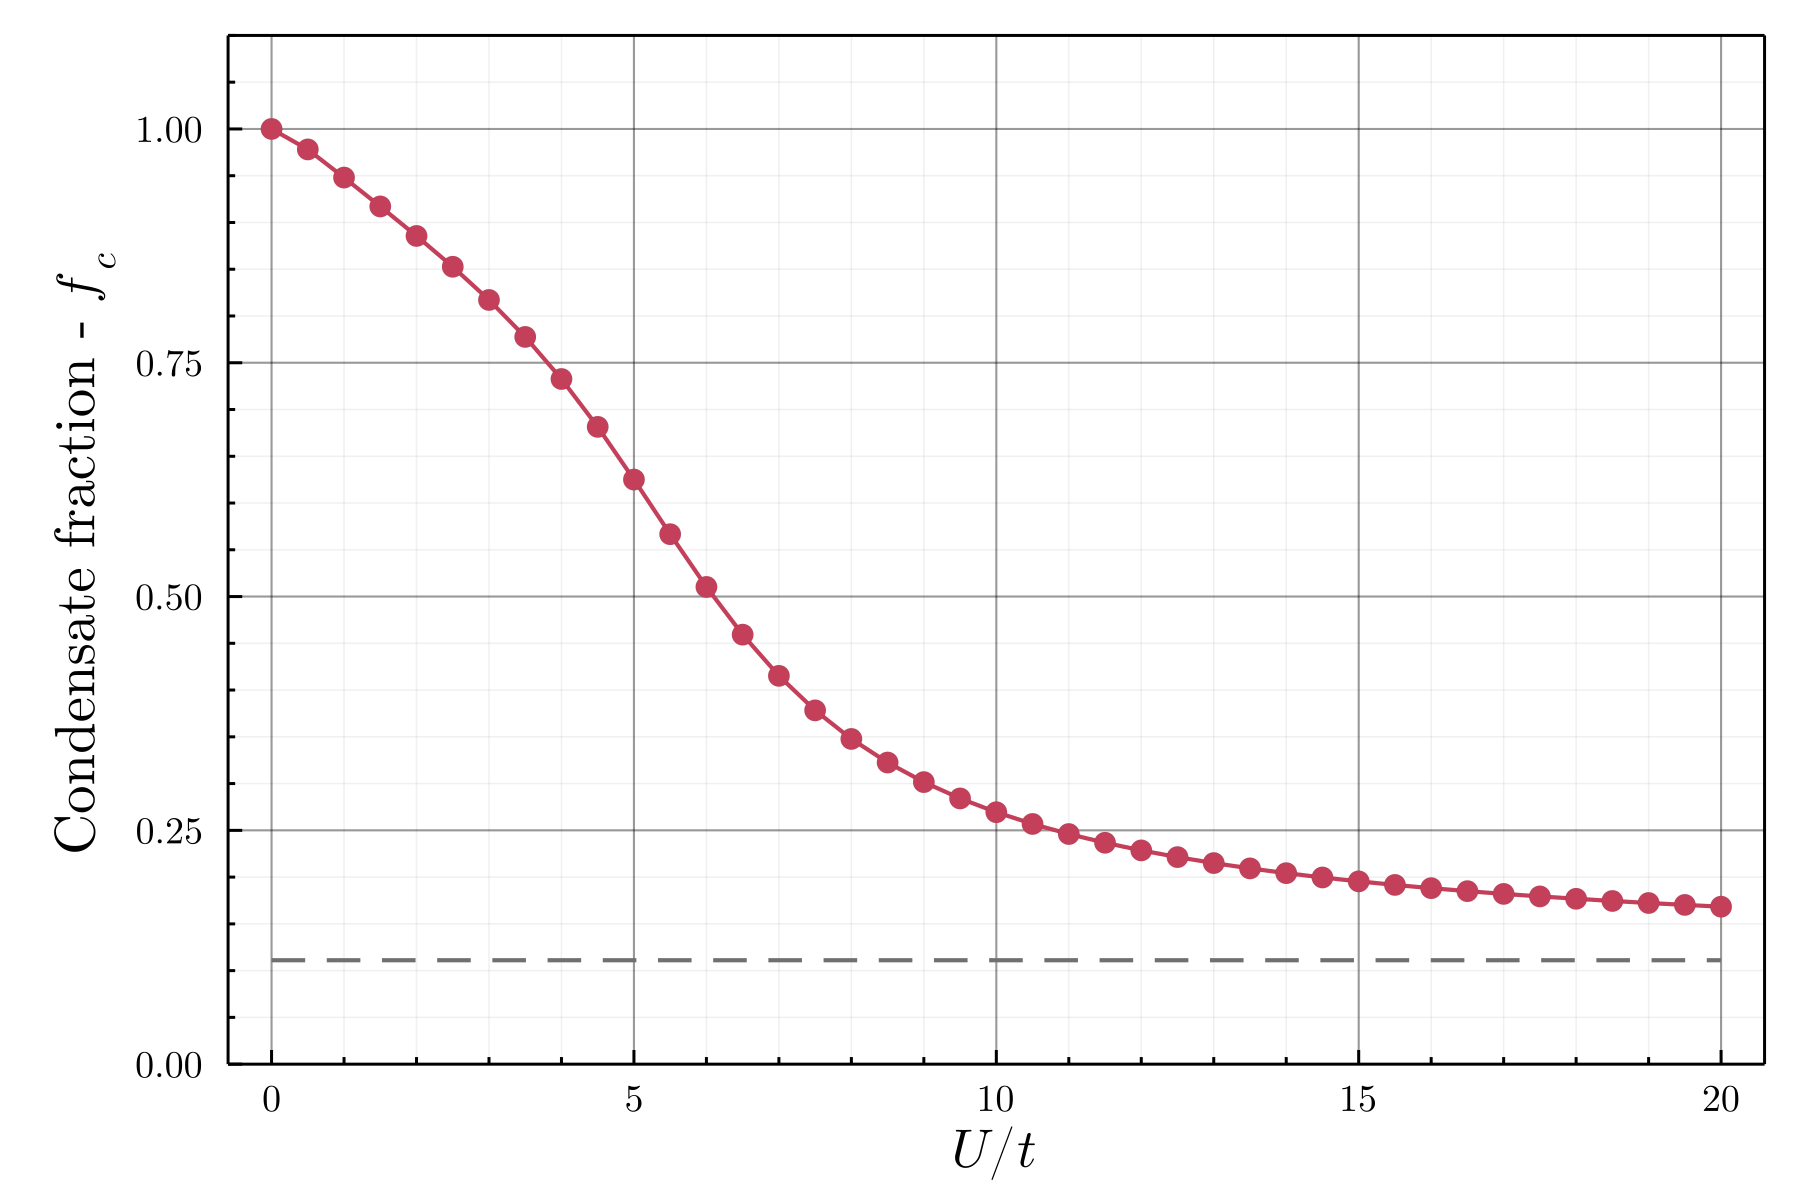
\includegraphics[width=\textwidth]{ch4/condensate_fraction.png}
        \caption{Condensate fraction}
        \label{fig:cond_frac}
    \end{subfigure}
    \hspace{1em}  %\hfill
    \begin{subfigure}[b]{0.45\textwidth}
        \centering
        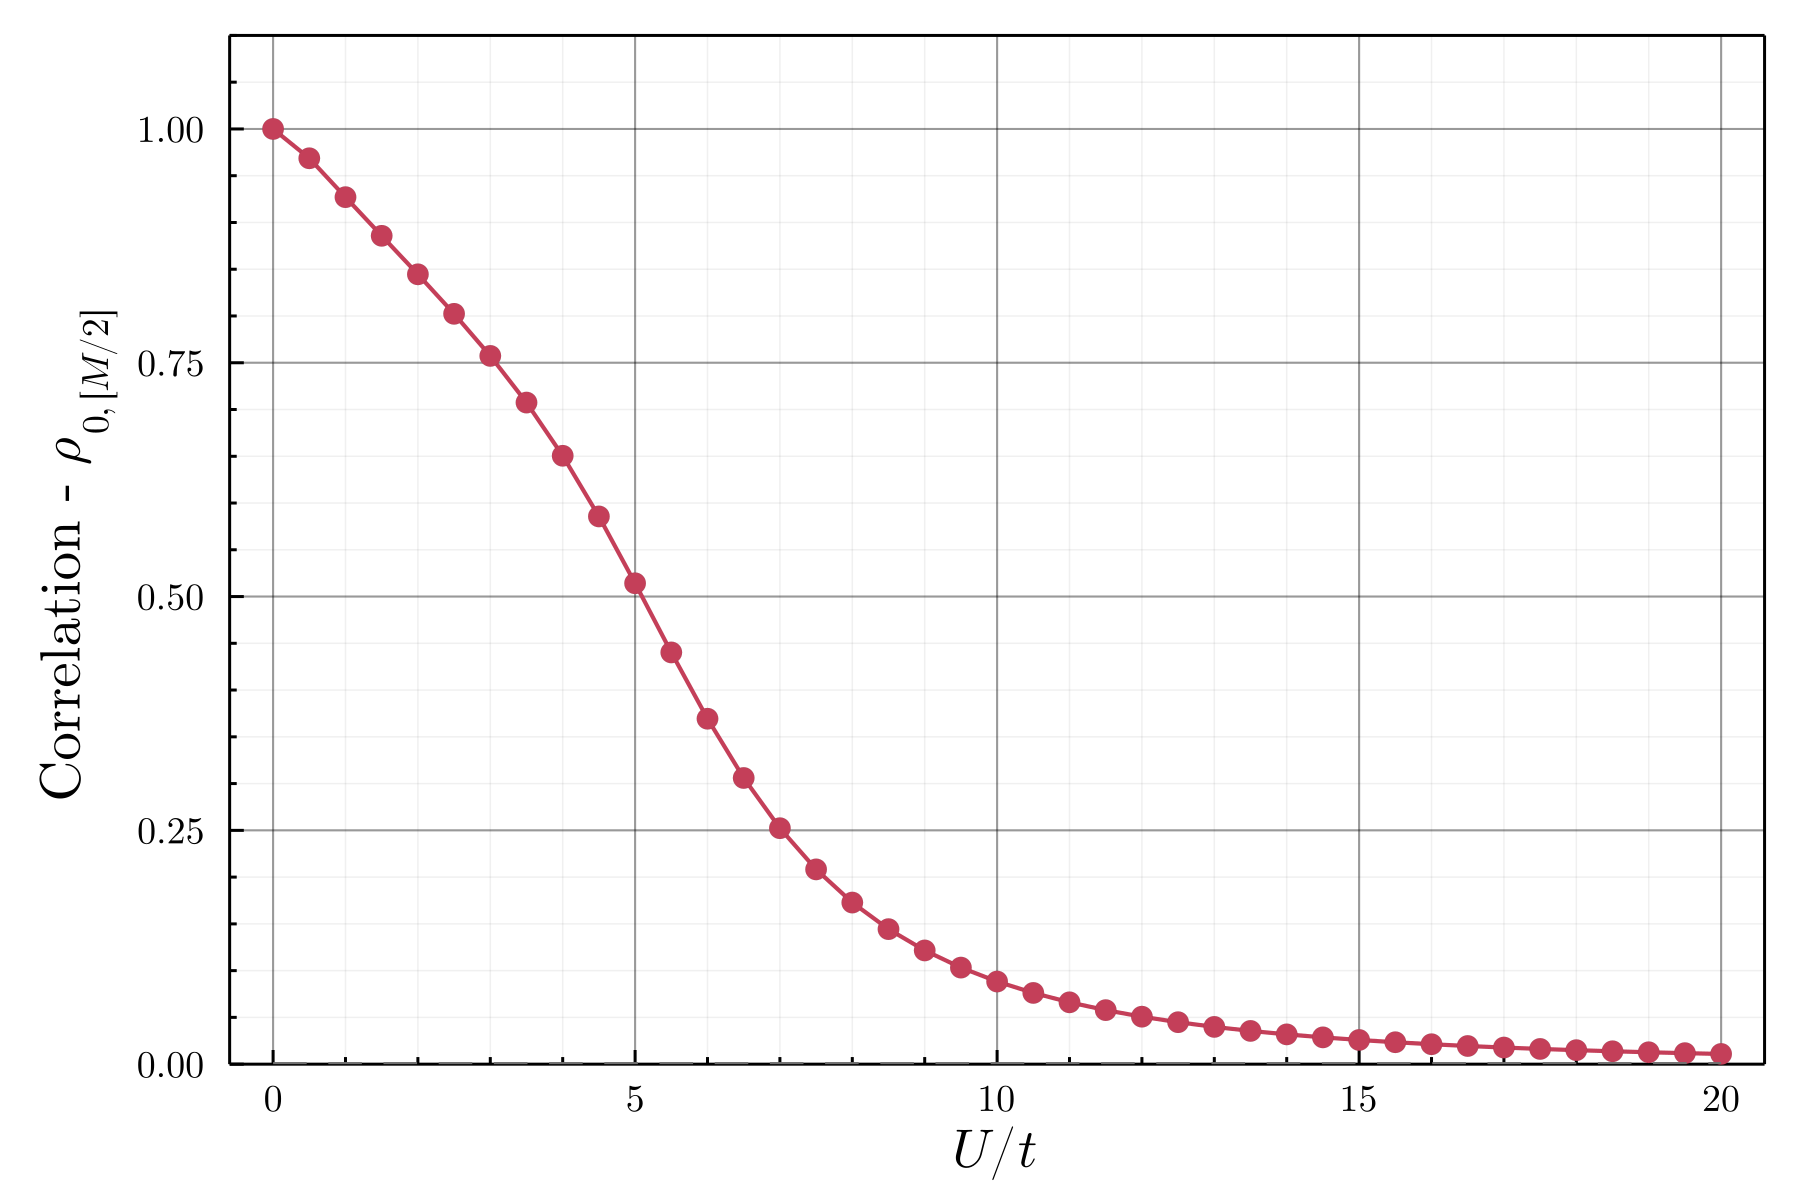
\includegraphics[width=\textwidth]{ch4/odlro.png}
        \caption{Off-diagonal Long-range order}
        \label{fig:odlro}
    \end{subfigure}
    \caption{Tracking the phase transition using various observables ($N = M = 9$)}
    \label{fig:ed_track}
\end{figure}
%%% FIG %%%
\FloatBarrier \!\!\!\!\!\!\!\!\!\!\!

We see in Fig. \ref{fig:cond_frac} that the condensate fraction, $f$, quickly drops from $1$ as $U/t$ is increased. However, note that it never vanishes even for arbitrarily small $U/t$, against our expectations for the Mott insulator phase. This turns out to be an artifact of the finite size of the system. Since the eigenvalues of the SPDM must satisfy $n_0 \geq 1$, we have $f \geq 1/M$ which would vanish for large $M$. 
\vspace{0.5cm}\\
On the other hand, in Fig. \ref{fig:odlro} we have plotted the matrix element of the SPDM with the farthest indices, in an attempt to capture the ODLRO condition. Surprisingly, we do see that the element starts off at $1$ and quickly vanishes in the Mott insulator regime, even though the condition of $|i-j| \to \infty$ cannot really be achieved in such a small system.
\vspace{0.5cm}\\
There is also another observable that is worth tracking, namely, the average variance of the number operator on an arbitrary lattice site, $\langle \delta n^2\rangle$. Since the Mott insulator phase is expected to be a pure Fock state, the occupation variance must vanish. 

%%% FIG %%%
\begin{figure}[!htb]
    \centering
    \begin{subfigure}[b]{0.52\textwidth}  %keep total sum <1 to show in same line
        \centering
        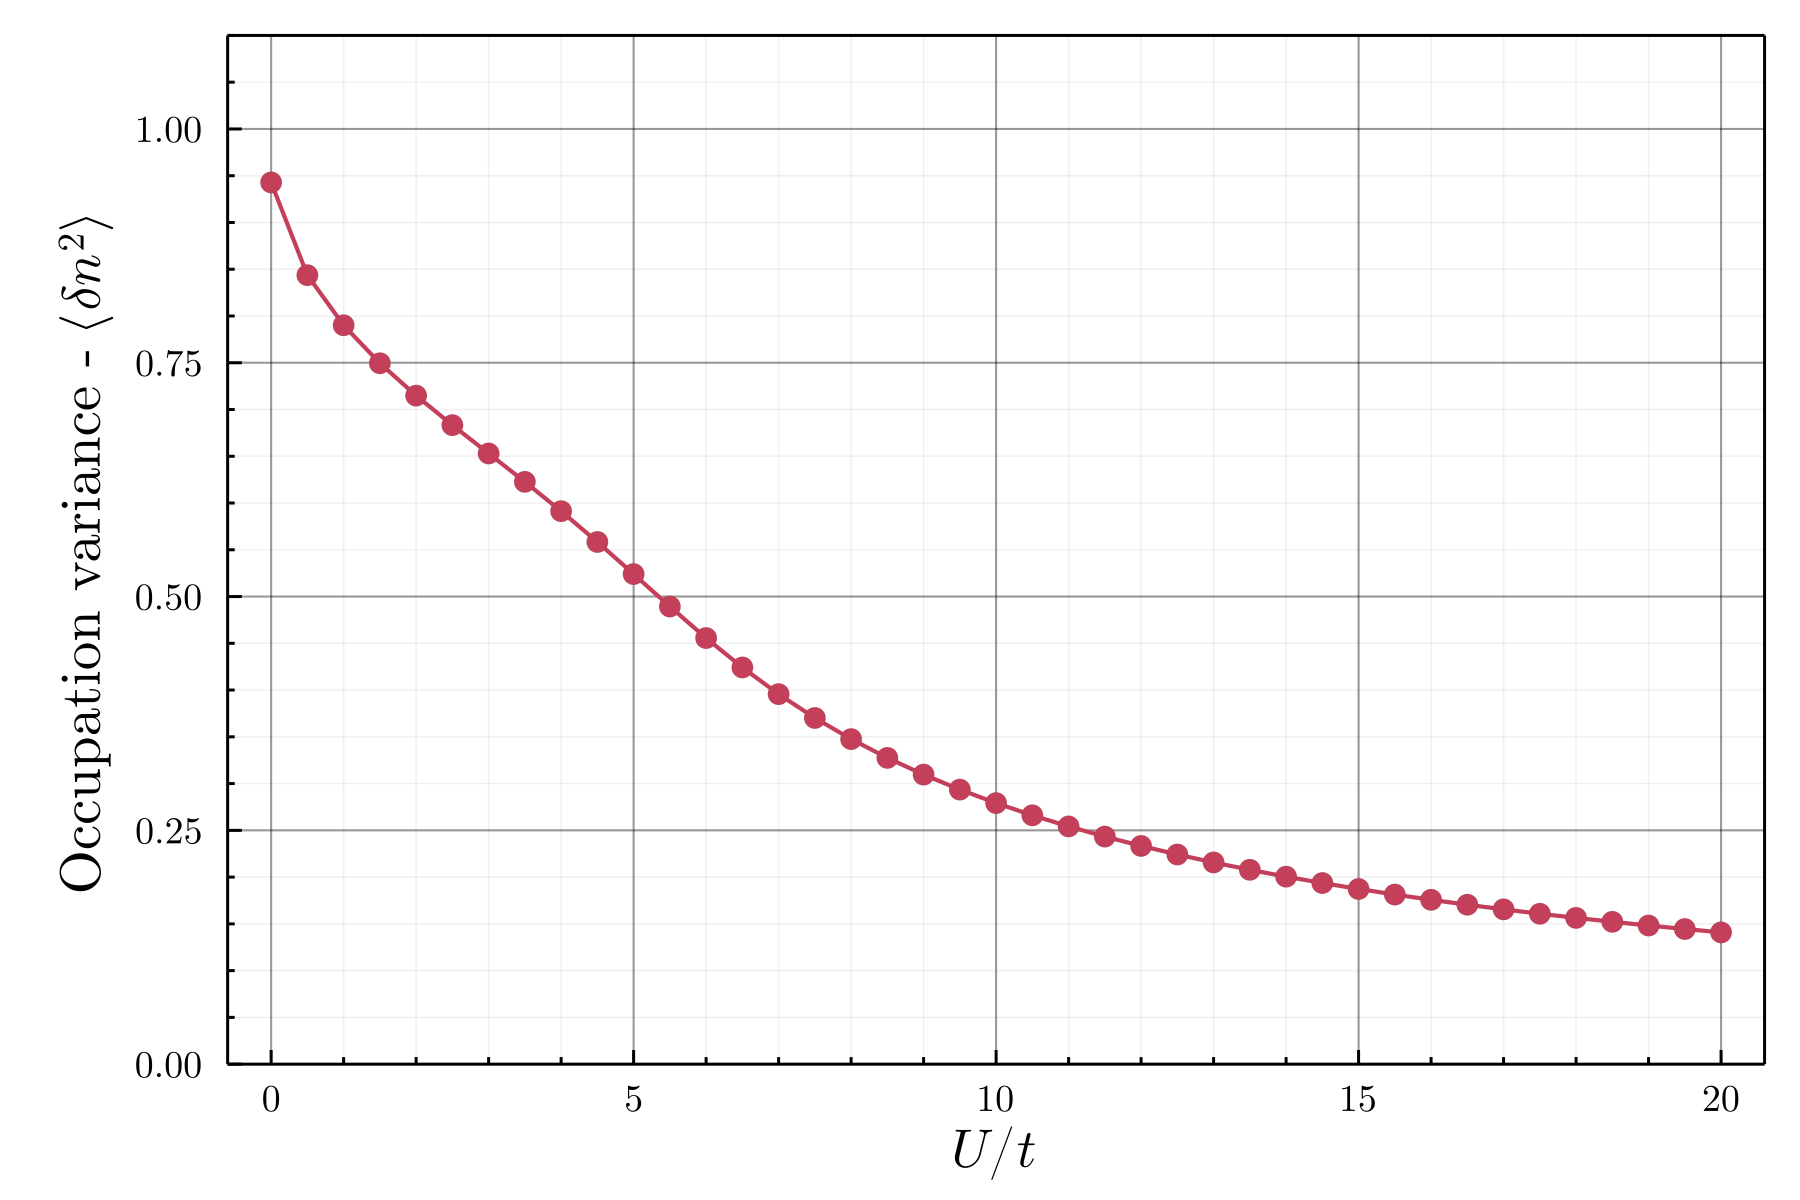
\includegraphics[width=\textwidth]{ch4/occupation_var.png}
        \caption{Canonical ensemble $(N=9, M=9)$}
        \label{fig:occ_var}
    \end{subfigure}
    \hspace{1em}  %\hfill
    \begin{subfigure}[b]{0.38\textwidth}
        \centering
        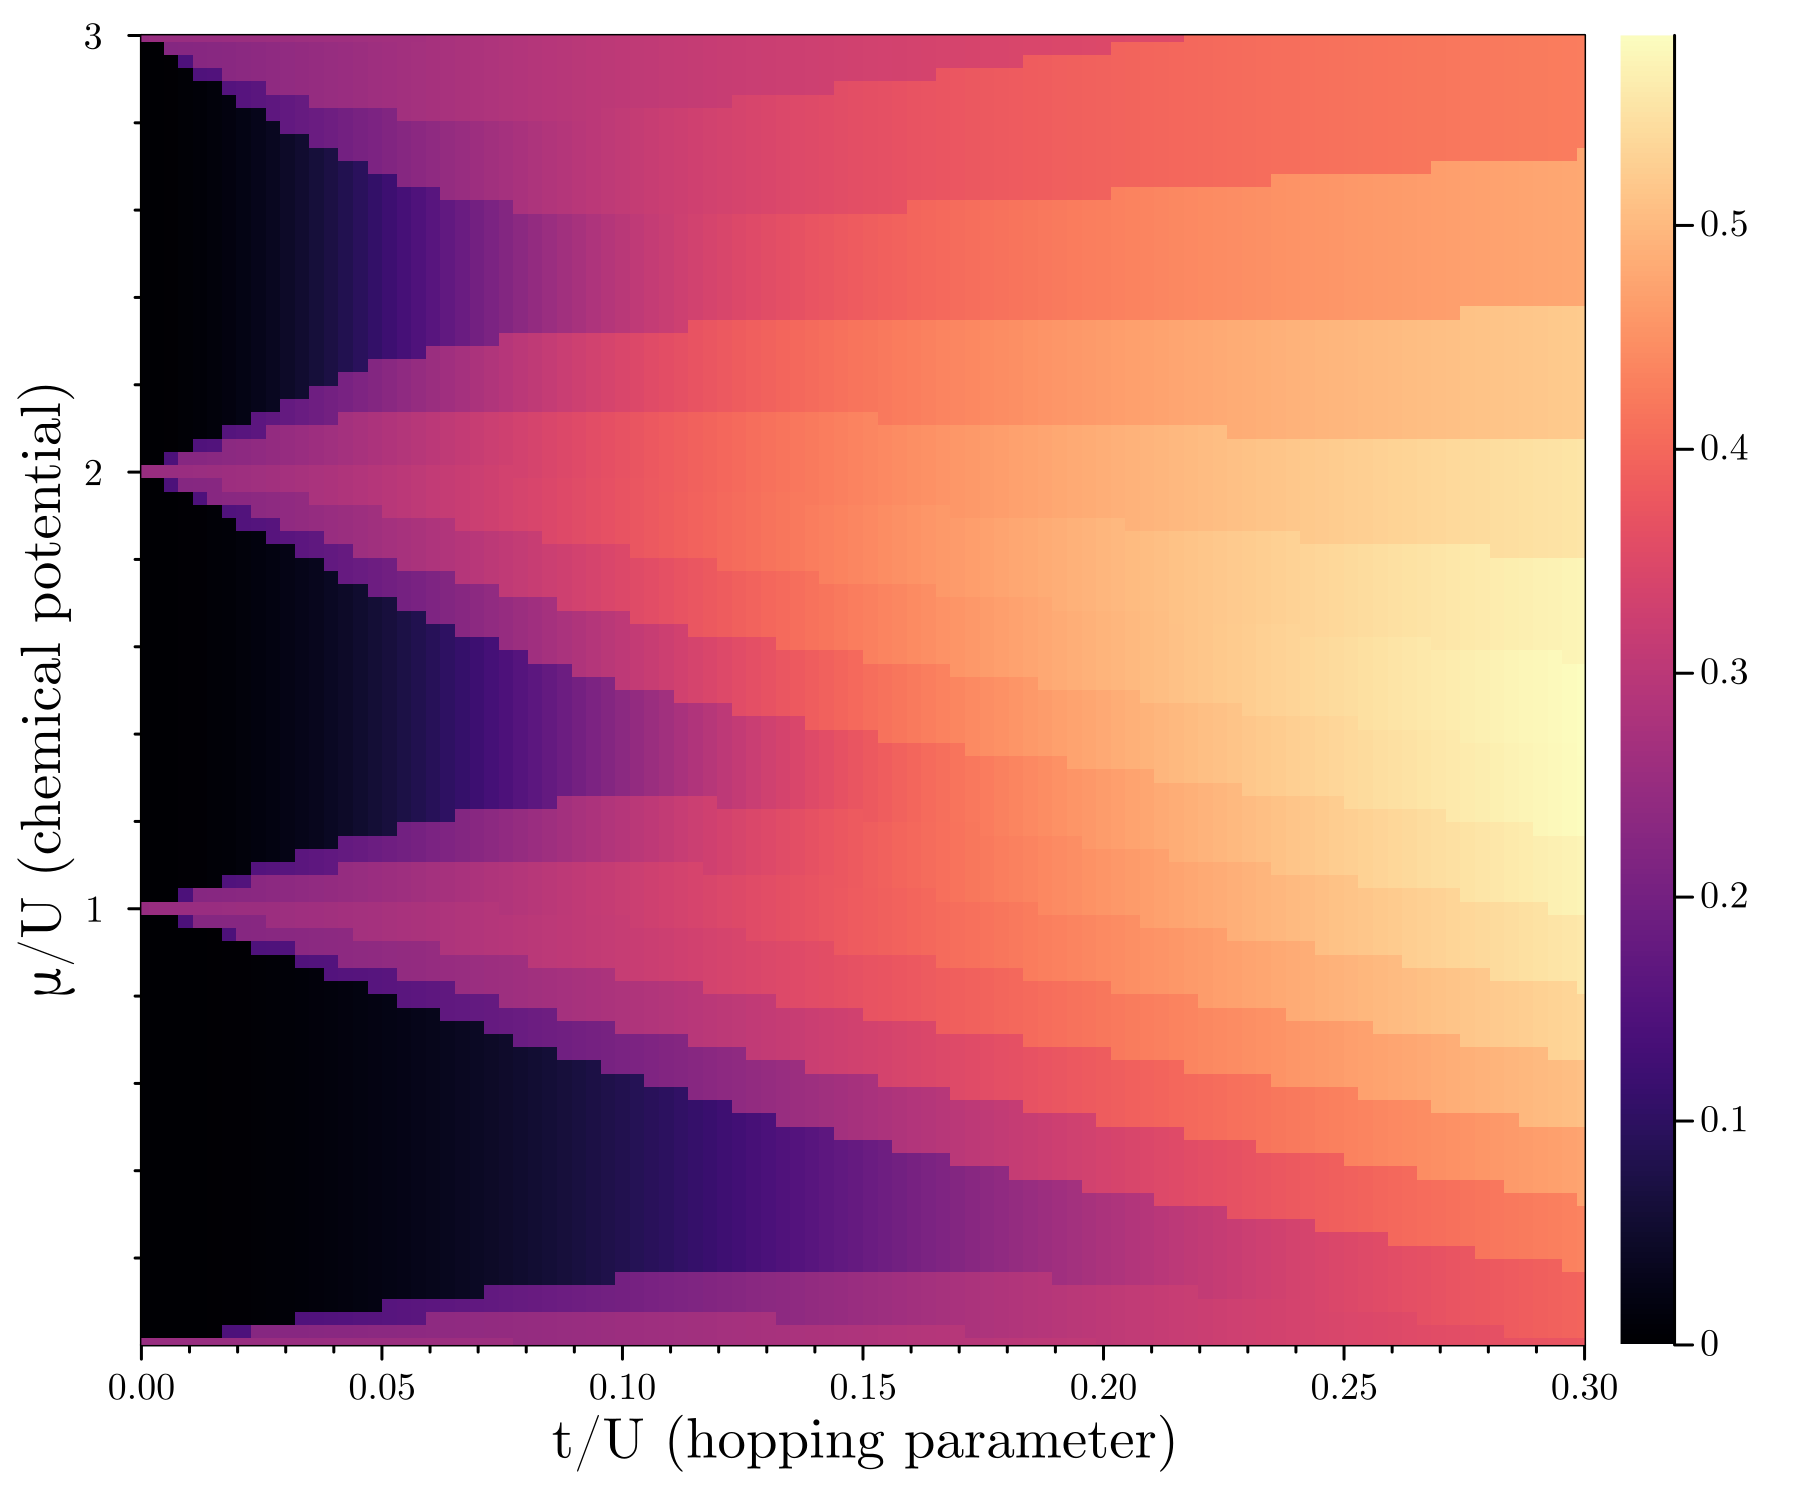
\includegraphics[width=\textwidth]{ch4/phase_diagram_ed.png}
        \caption{ Grand canonical ensemble $(N_{max} = 4, M = 6)$}
        \label{fig:phasediagram_ed}
    \end{subfigure}
    \caption{Tracking the phase transition using average variance of occupation number}
    \label{}
\end{figure}
%%% FIG %%%
\FloatBarrier \!\!\!\!\!\!\!\!\!\!\!

Unsurprisingly, Fig. \ref{fig:occ_var}, also demonstrates a curve with a similar trend as the ones in Fig. \ref{fig:ed_track}. Although there seems to be some signatures of the quantum phase transition, it seems that the Mott insulator phase strictly only exists for $U/t \to \infty$  ($\implies t/U = 0$). However, note that these results were obtained from an exact diagonalization over a fixed-$N$ subspace of the Fock space. If we allow variable particle number (upto an arbitrary cut-off, $N \in [0, N_{max}]$) by considering a grand canonical ensemble instead, we can gain some more insight. We see that this is indeed the case, as the phase diagram obtained in Fig. \ref{fig:phasediagram_ed} suggests that the Mott insulator phase could exist in an extended region away from $t/U = 0$.
\vspace{0.5cm}\\
However, it is dubious to make this claim rigorously since all of our possible order parameters are muddled by the finite (and small!) lattice size that we have considered. One could extend this analysis by exactly diagonalizing a larger system, however, the computational cost increases exponentially and quickly becomes unfeasible after $\sim 20$ sites. Instead, we will proceed to explore some approximate methods that allow us to get more qualitative but well-defined results. 

\section{Mean Field Theory}\label{sec:bhm_mft}
The motivation for this technique is the fact that diagonalizing the BHM in either of the extreme limits is trivial, however the dimensionality of the Hilbert space blows up in the general case, Eq. \eqref{eq:bhm1}. Note that we will continue working exclusively in the grand canonical ensemble. 
%%% FIG %%%
\begin{figure}[!htb]
    \centering
    \begin{subfigure}[b]{\textwidth}  %keep total sum <1 to show in same line
        \centering
        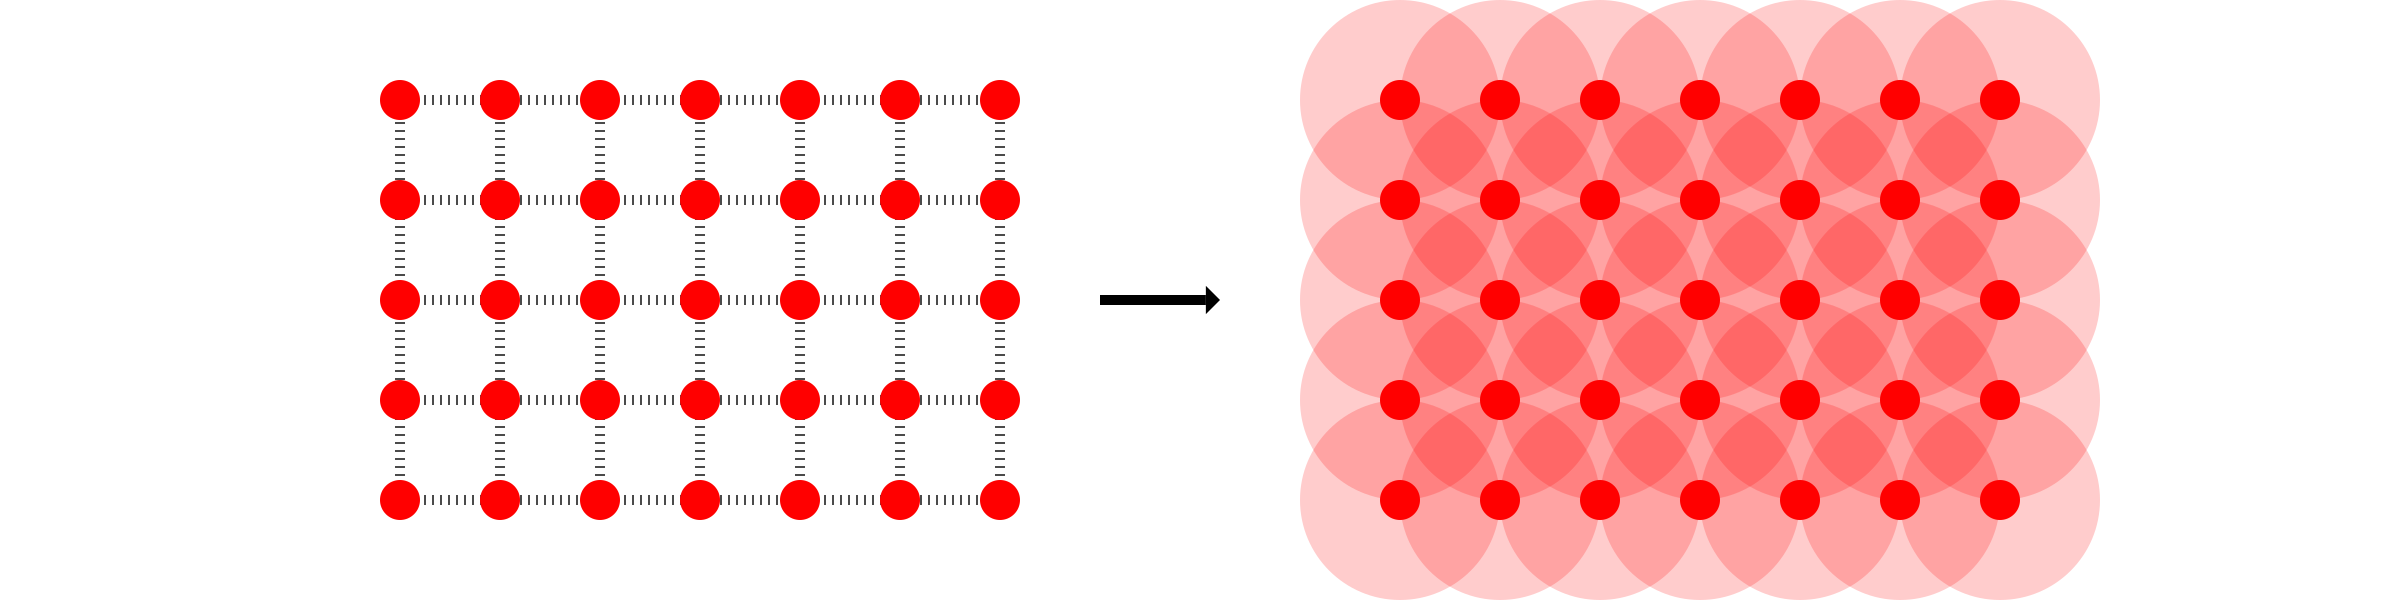
\includegraphics[width=\textwidth]{ch4/MFTdiagram.png}
    \end{subfigure}
    \caption{Pictorial representation of MFT in 2D}
    \label{}
\end{figure}
%%% FIG %%%
\FloatBarrier \!\!\!\!\!\!\!\!\!\!\!

In order to extract some qualitative features of the model, we attempt a de-coupling which results in a system with a smaller Hilbert space. To facilitate this, we will replace the site operators with their expectation values and ignore the higher order fluctations.
\begin{align}\label{eq:decoupling_scheme}
    &\hspace{1.2cm}\hat{a}_i = \Psi_i + \delta \hat{a}_i \nonumber \\
    &\implies \delta a_i^{\dagger} \delta a_j = (a_i^{\dagger} - \Psi_i^*)(a_j - \Psi_j) \approx 0 \nonumber \\
    &\implies a_i^{\dagger}a_j \approx \Psi_ja_i^{\dagger} + \Psi_i^*a_j - \Psi_i^*\Psi_j
\end{align}

We can now de-couple the hopping term like so:
\begin{align}
    -H_{hop}/t &= \sum_{\langle i, j\rangle} a_i^{\dagger}a_j \nonumber \\
    &= \sum_{\langle i, j\rangle} (\Psi_ja_i^{\dagger} + \Psi_i^*a_j - \Psi_i^*\Psi_j)\nonumber \\
    &= \sum_i \big (\sum_{j \in N_i} \Psi_j\big ) a_i^{\dagger} + \sum_i \big (\sum_{j \in N_i} \Psi_j^*\big ) a_i - \sum_i \big (\sum_{j \in N_i} \Psi_j\big) \Psi_i^*
\end{align}

where $N_i$ is the set of nearest neighbour indices for the lattice site $i$. Defining the mean order parameter, $\overline{\Psi}_i = \frac{1}{z}\sum_{j \in N_i} \Psi_j$,  where $z$ is the coordination number of the lattice, we obtain:
\begin{align}\label{eq:mft_hop}
    -H_{hop}/zt = \sum_i (\overline{\Psi}_i a_i^{\dagger} + \overline{\Psi}_i^* a_i - \overline{\Psi}_i\Psi_i^*)
\end{align}
We can then write the entire site-decoupled Hamiltonian which depends on a set of $M$ mean-field parameters, $\{\Psi_i\}$ as follows.
\begin{equation}
    H_{MF}\{\Psi_i\} = \sum_i H_i\{\Psi_i\}
\end{equation}
\begin{equation}\label{eq:mft}
    H_i\{\Psi_i\} = -zt(\overline{\Psi}_i a_i^{\dagger} + \overline{\Psi}_i^* a_i - \overline{\Psi}_i\Psi_i^*) + \frac{U}{2}n_i(n_i - 1) - \mu n_i
\end{equation}

The complexity of the problem is drastically reduced now that we only have to solve $M$ single-site Hamiltonians. Such a mean-field decoupling effectively proposes the following product ansatz for the wavefunction:
\begin{equation}
    \ket{\Psi} = \bigotimes_{i = 1}^M (\sum_{n = 0}^{\infty} f_{i, n} \ket{n})
\end{equation}
This is in-fact equivalent to the Gutzwiller Mean-field approach\cite{Jaksch_1998}, wherein the co-efficients $f_{i, n}$ are obtained such that the free energy is minimized. We will however utilize a self-consistent scheme to obtain the ground state solution.
\vspace{0.5cm}\\
We can further simplify the Hamiltonian by setting $\Psi_i = \Psi$ due to the translational symmetry of the system. It then follows that $\overline{\Psi} = \Psi$. Further, due to the $U(1)$ symmetry (invariance under a global phase shift, $\hat{a}_i \rightarrow e^{i\theta}\hat{a}_i$) of the BHM, we can assume that $\Psi \in \mathbb{R}$ without loss of generality.
\begin{equation}\label{eq:bhm_mft}
      H_i\{\Psi\} = -zt\Psi (a_i + a_i^{\dagger}) + \frac{U}{2} n_i(n_i -1) - \mu n_i + zt|\Psi|^2
\end{equation}


\subsection{Numerical solution}
Since all the single-site Hamiltonians are equivalent, it is sufficient to solve any one of them and we will drop the index $i$ henceforth. It now seems that we can trivially diagonalize $H\{\Psi\}$ to study the system. However, there are still a few considerations to be made. 
\vspace{0.5cm}\\
Firstly, in order to construct the matrix form of $H\{\Psi\}$, the local number basis $(\{\ket{n}\}|_{n = 0}^{\infty})$ seems to be an obvious choice. However, this would give rise to an infinite dimensional matrix, so we must choose to truncate the basis at some $n_{max}$. We will discuss this further in Sec. \ref{sec:nmax}.
\vspace{0.5cm}\\
Secondly, $H\{\Psi\}$ is parametrized by the mean-field parameter, $\Psi$, which is required to construct the matrix. But by definition, we have $\Psi = \bra{\psi_{gs}}\hat{a}\ket{\psi_{gs}}$ which can only be computed by diagonalizing the Hamiltonian. Thus, the parameter $\Psi$ must be determined in a self-consistent manner. This can be described formally by wrapping this procedure into a function.
\begin{equation}\label{eq:self_fn}
    f(\Psi) \rightarrow \text{Diagonalize } H\{\Psi\} \text{ and compute } \psi_{gs} \rightarrow \bra{\psi_{gs}}\hat{a}\ket{\psi_{gs}}
\end{equation}
Solving the self-consistency loop is equivalent to finding the fixed point $\Psi^*$ such that $f(\Psi^*) = \Psi^*$. One can now utilize the machinery of non-linear dynamics and root-finding techniques to solve this problem.
\vspace{0.5cm}\\
The most direct (and ubiquitous) method to proceed with is Fixed Point Iteration. This involves starting with an initial guess $\Psi^{(0)}$, and computing $\Psi^{(n)} = f(\Psi^{(n-1)})$ repeatedly until it converges within a specified tolerance. Such a method can be highly sensitive to the choice of initial guess, and there is no guarantee of convergence nor a bound on how fast it happens. However, these issues can be ignored for now and do not crop up until a later point (see Sec. \ref{sec:caveats}).

\subsection{Plotting the phase diagram}
Before we proceed, it is important to note that the mean-field Hamiltonian clearly changes certain features of the original Hamiltonian. A striking example of this is that while Eq. \ref{eq:bhm1} conserves the particle number, Eq. \ref{eq:mft} does not! It seems then that our 'choice' of working in the grand canonical ensemble is strictly necessary at the mean-field level. At this point, we must ask whether such a Hamiltonian can still admit phases that can be classified as a Mott insulator or a superfluid.

\begin{figure}[!htb]
    \centering
    \begin{subfigure}[b]{0.48\textwidth}  %keep total sum <1 to show in same line
        \centering
        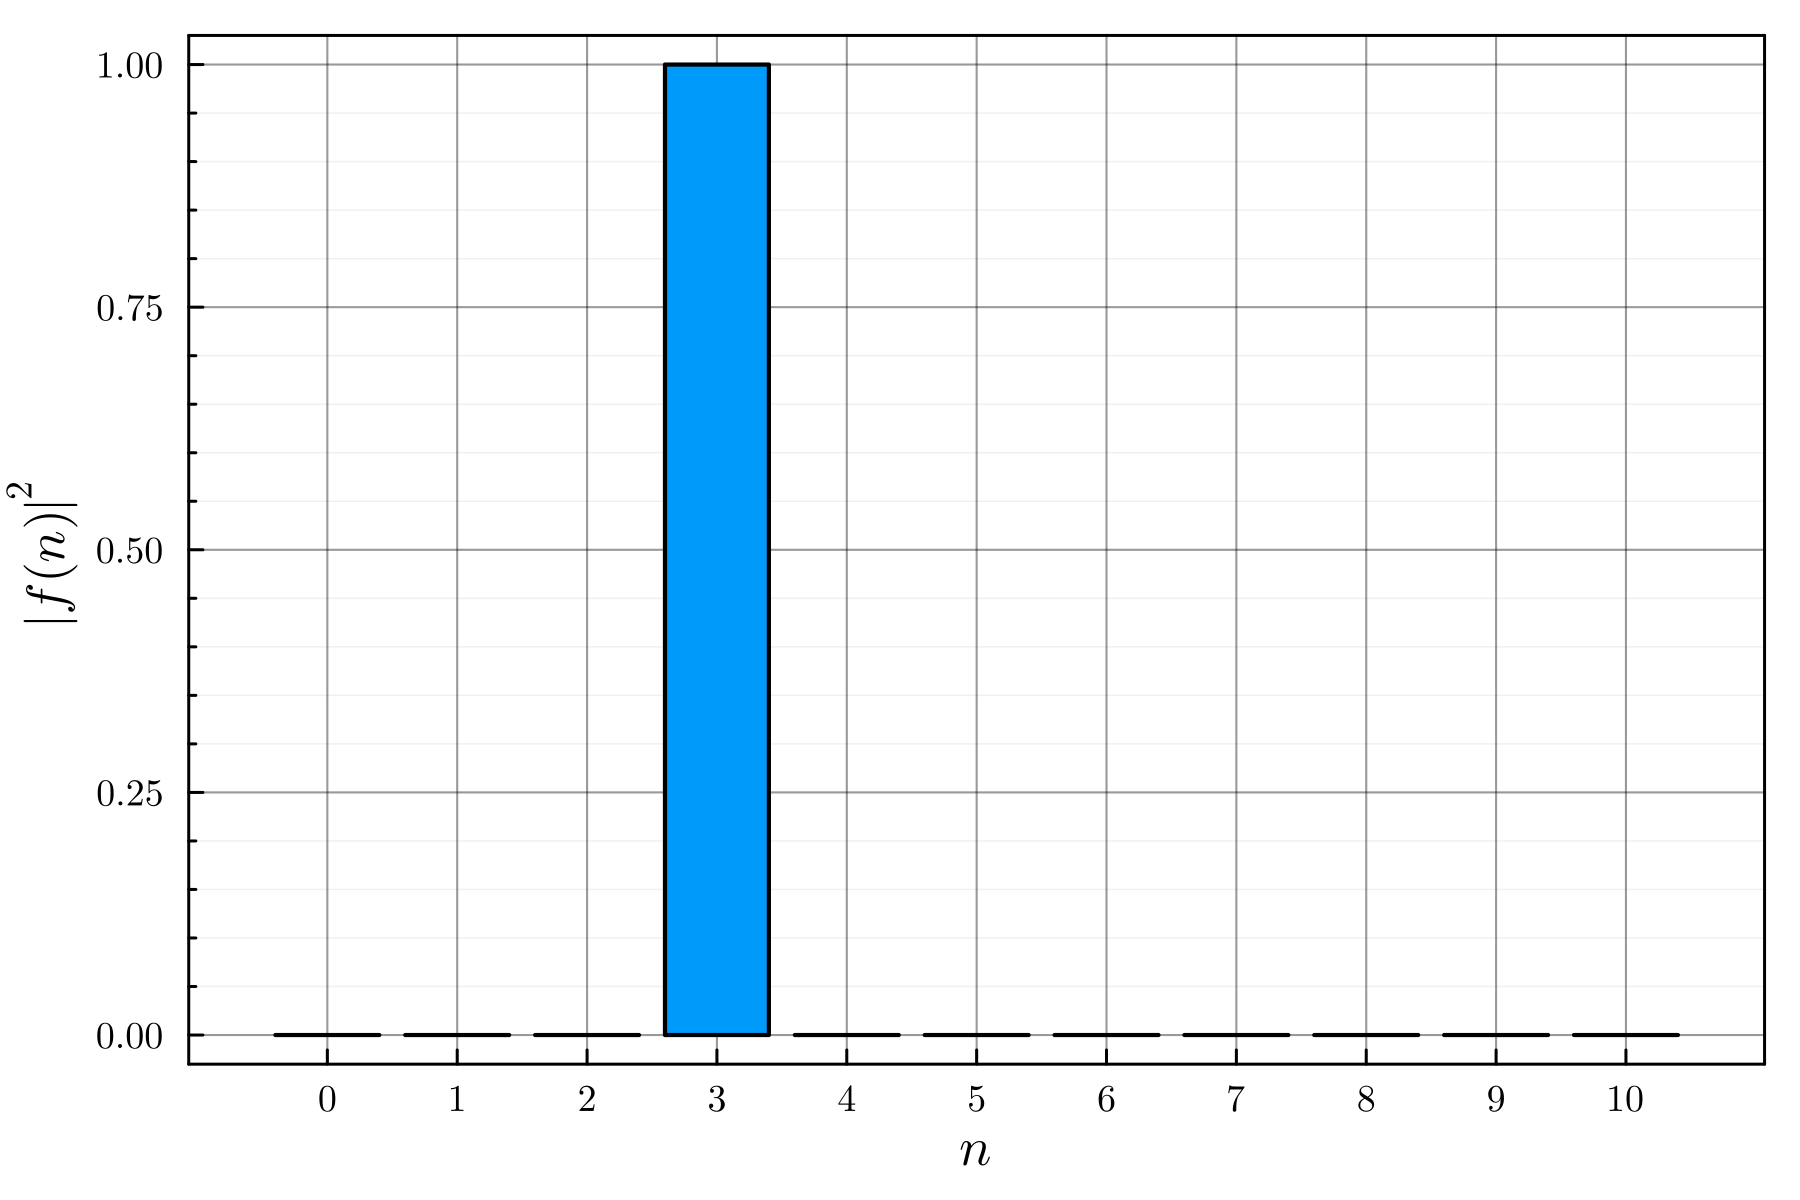
\includegraphics[width=\textwidth]{ch4/MI_dist.png}
        \caption{Mott insulator; $t = 0.01, \mu = 2.5$, $U = 1$}
        \label{fig:mi_dist}
    \end{subfigure}
    \hspace{1em}  %\hfill
    \begin{subfigure}[b]{0.48\textwidth}
        \centering
        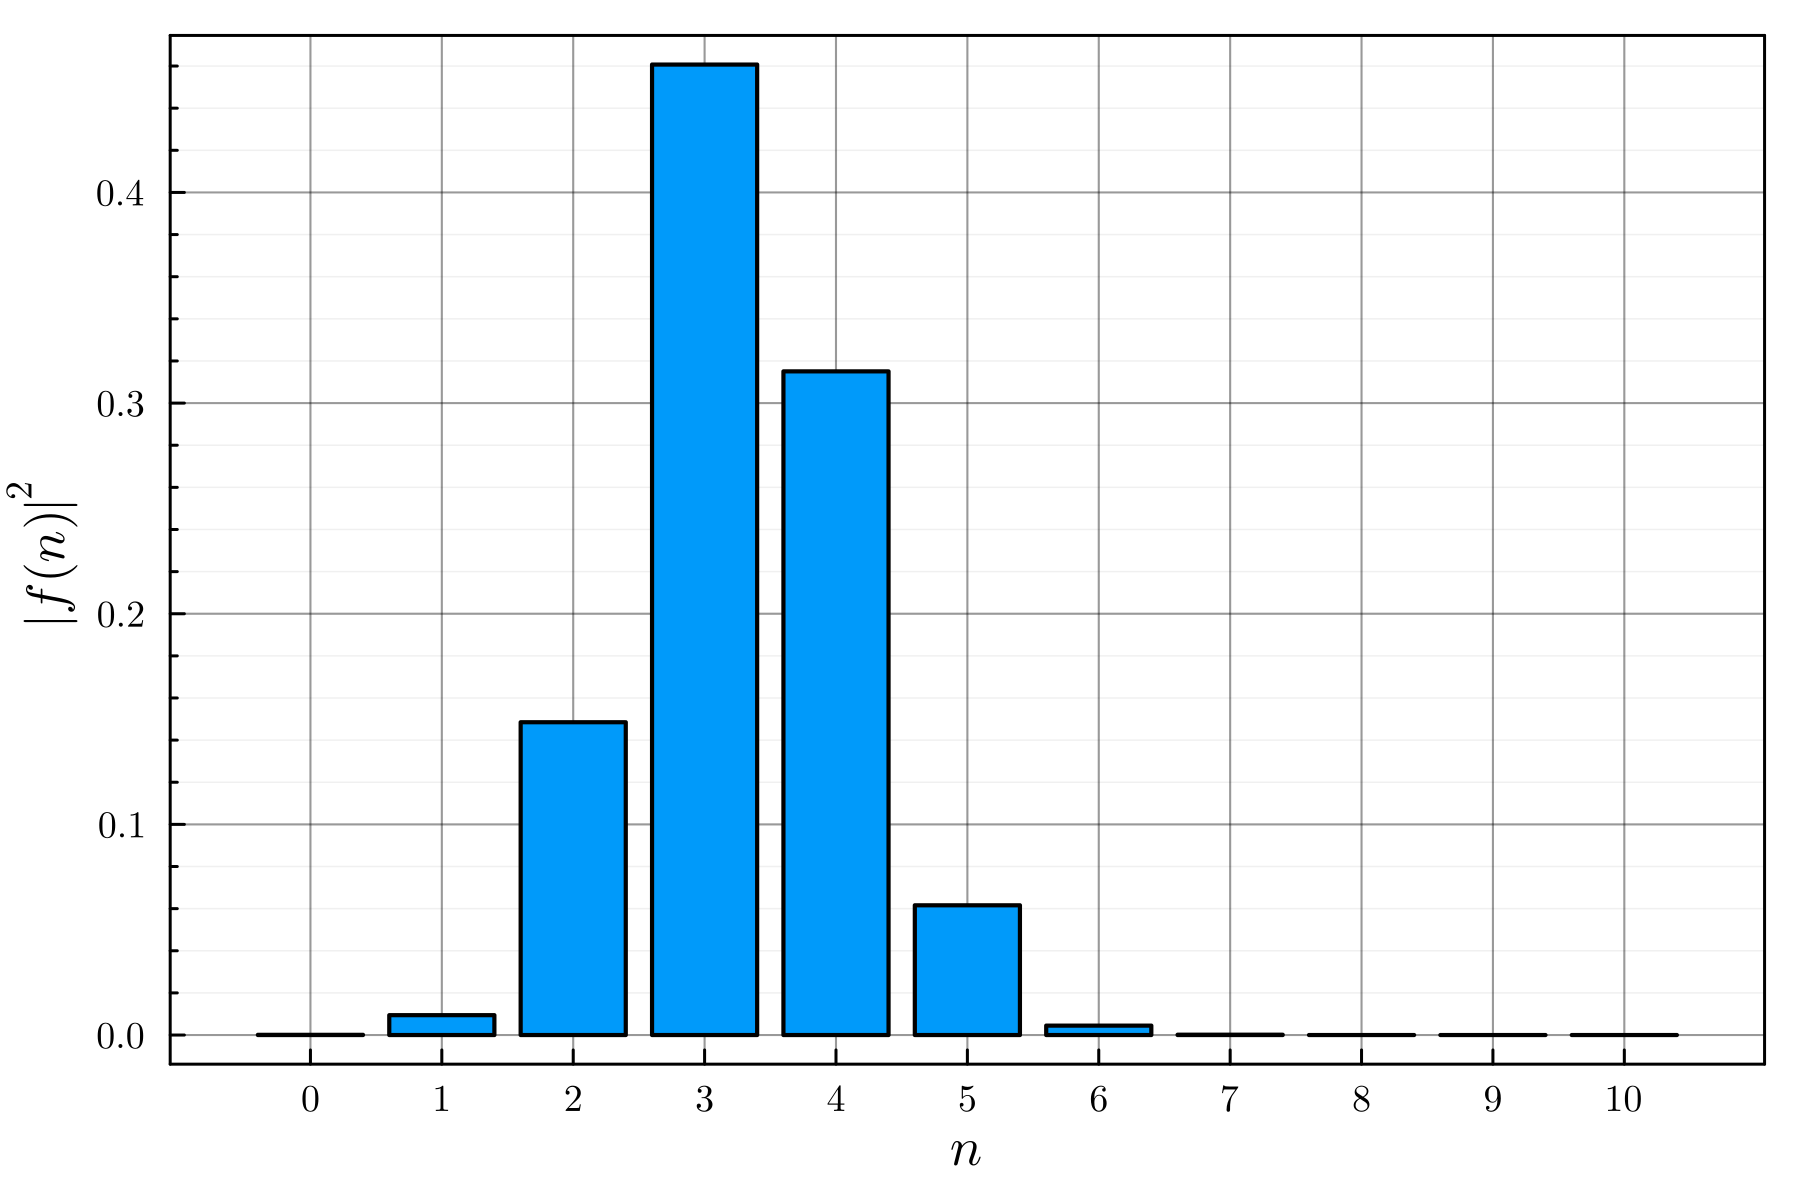
\includegraphics[width=\textwidth]{ch4/SF_dist.png}
        \caption{Superfluid; $t = 0.2, \mu = 2.5$, $U = 1$}
        \label{fig:sf_dist}
    \end{subfigure}
    \caption{Distribution of co-efficients in Fock basis}
    \label{fig:dists}
\end{figure}
%%% FIG %%%
\FloatBarrier \!\!\!\!\!\!\!\!\!\!\!

Solving the mean-field Hamiltonian for various parameter choices results in two distinct phases as seen in Fig. \ref{fig:dists}. The Mott insulator phase is captured as a pure Fock state with fixed occupation number on each lattice site. On the other hand, the superfluid phase is captured as a product of coherent states, which is a well-known means of describing BECs\cite{leggett2008, annett2003}. This can also be understood as the ground state picking up a random phase, $e^{i\theta}$, due to spontaneous breaking of the $U(1)$ symmetry. Further, the idea of particle number conservation can be loosely recovered by considering the thermodynamic limit wherein $\sqrt{\langle \delta n^2 \rangle}/\langle n \rangle \to 0$ as $N, M \to \infty$. In case this explanation is unsatisfactory, there is a way to formulate this scheme without breaking number conservation\cite{leggett2008}, but the analysis becomes far more cumbersome.
\vspace{0.5cm}\\
Now that we have confirmed that the ground state can admit these phases, we require an order parameter to distinguish them. A simple quantity presents itself by considering the definition of off-diagonal long-range order from Eq. \eqref{eq:odlro} as a means of identifying BECs.
\begin{equation}
    \lim_{|i-j| \to \infty} \langle a_i^{\dagger}a_j\rangle = \lim_{|i-j| \to \infty} \langle a_i^{\dagger}\rangle \langle a_j\rangle = \Psi_i^* \Psi_j = |\Psi|^2 \neq 0
\end{equation}
Note that such a decoupling is only valid at the mean-field level. We can clearly see now that the idea of spontaneous $U(1)$ symmetry breaking is captured by this result. Thus, we can use the mean-field parameter $\Psi$ as the superfluid order parameter as well.
\vspace{0.5cm}\\
The phase diagram can now be naively generated by computing the ground-state solution and hence the order parameter over a grid of $\mu/U$ and $t/U$ values.

\begin{figure}[!htb]
    \centering
    \begin{subfigure}[b]{0.45\textwidth}  %keep total sum <1 to show in same line
        \centering
        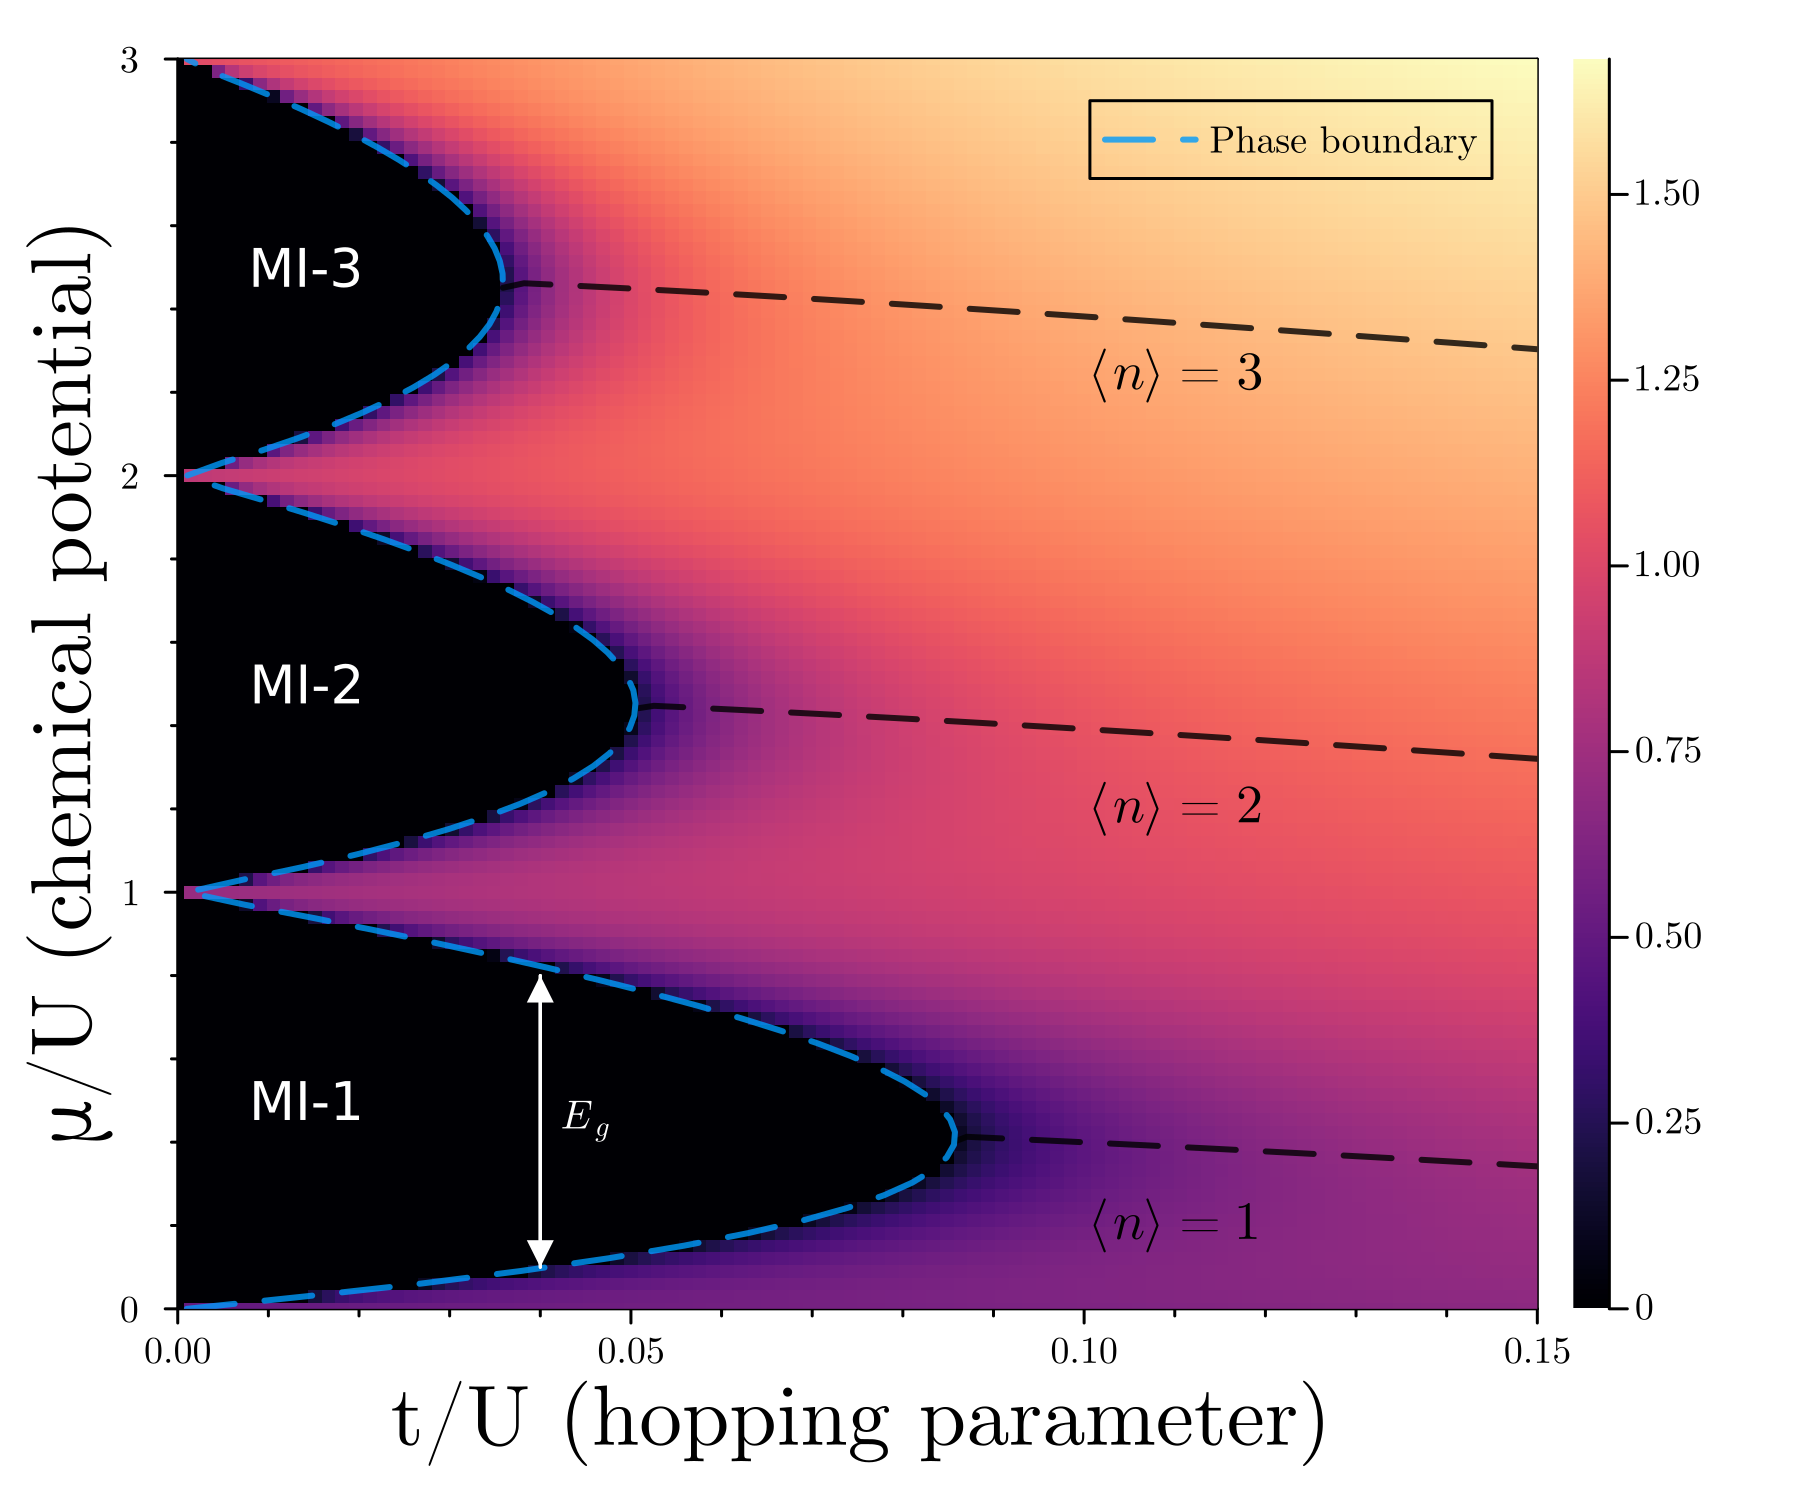
\includegraphics[width=\textwidth]{ch4/phase_diagram_op.png}
        \caption{Order parameter, $\langle a \rangle$}
        \label{fig:mft_pd}
    \end{subfigure}
    \hspace{1em}  %\hfill
    \begin{subfigure}[b]{0.45\textwidth}
        \centering
        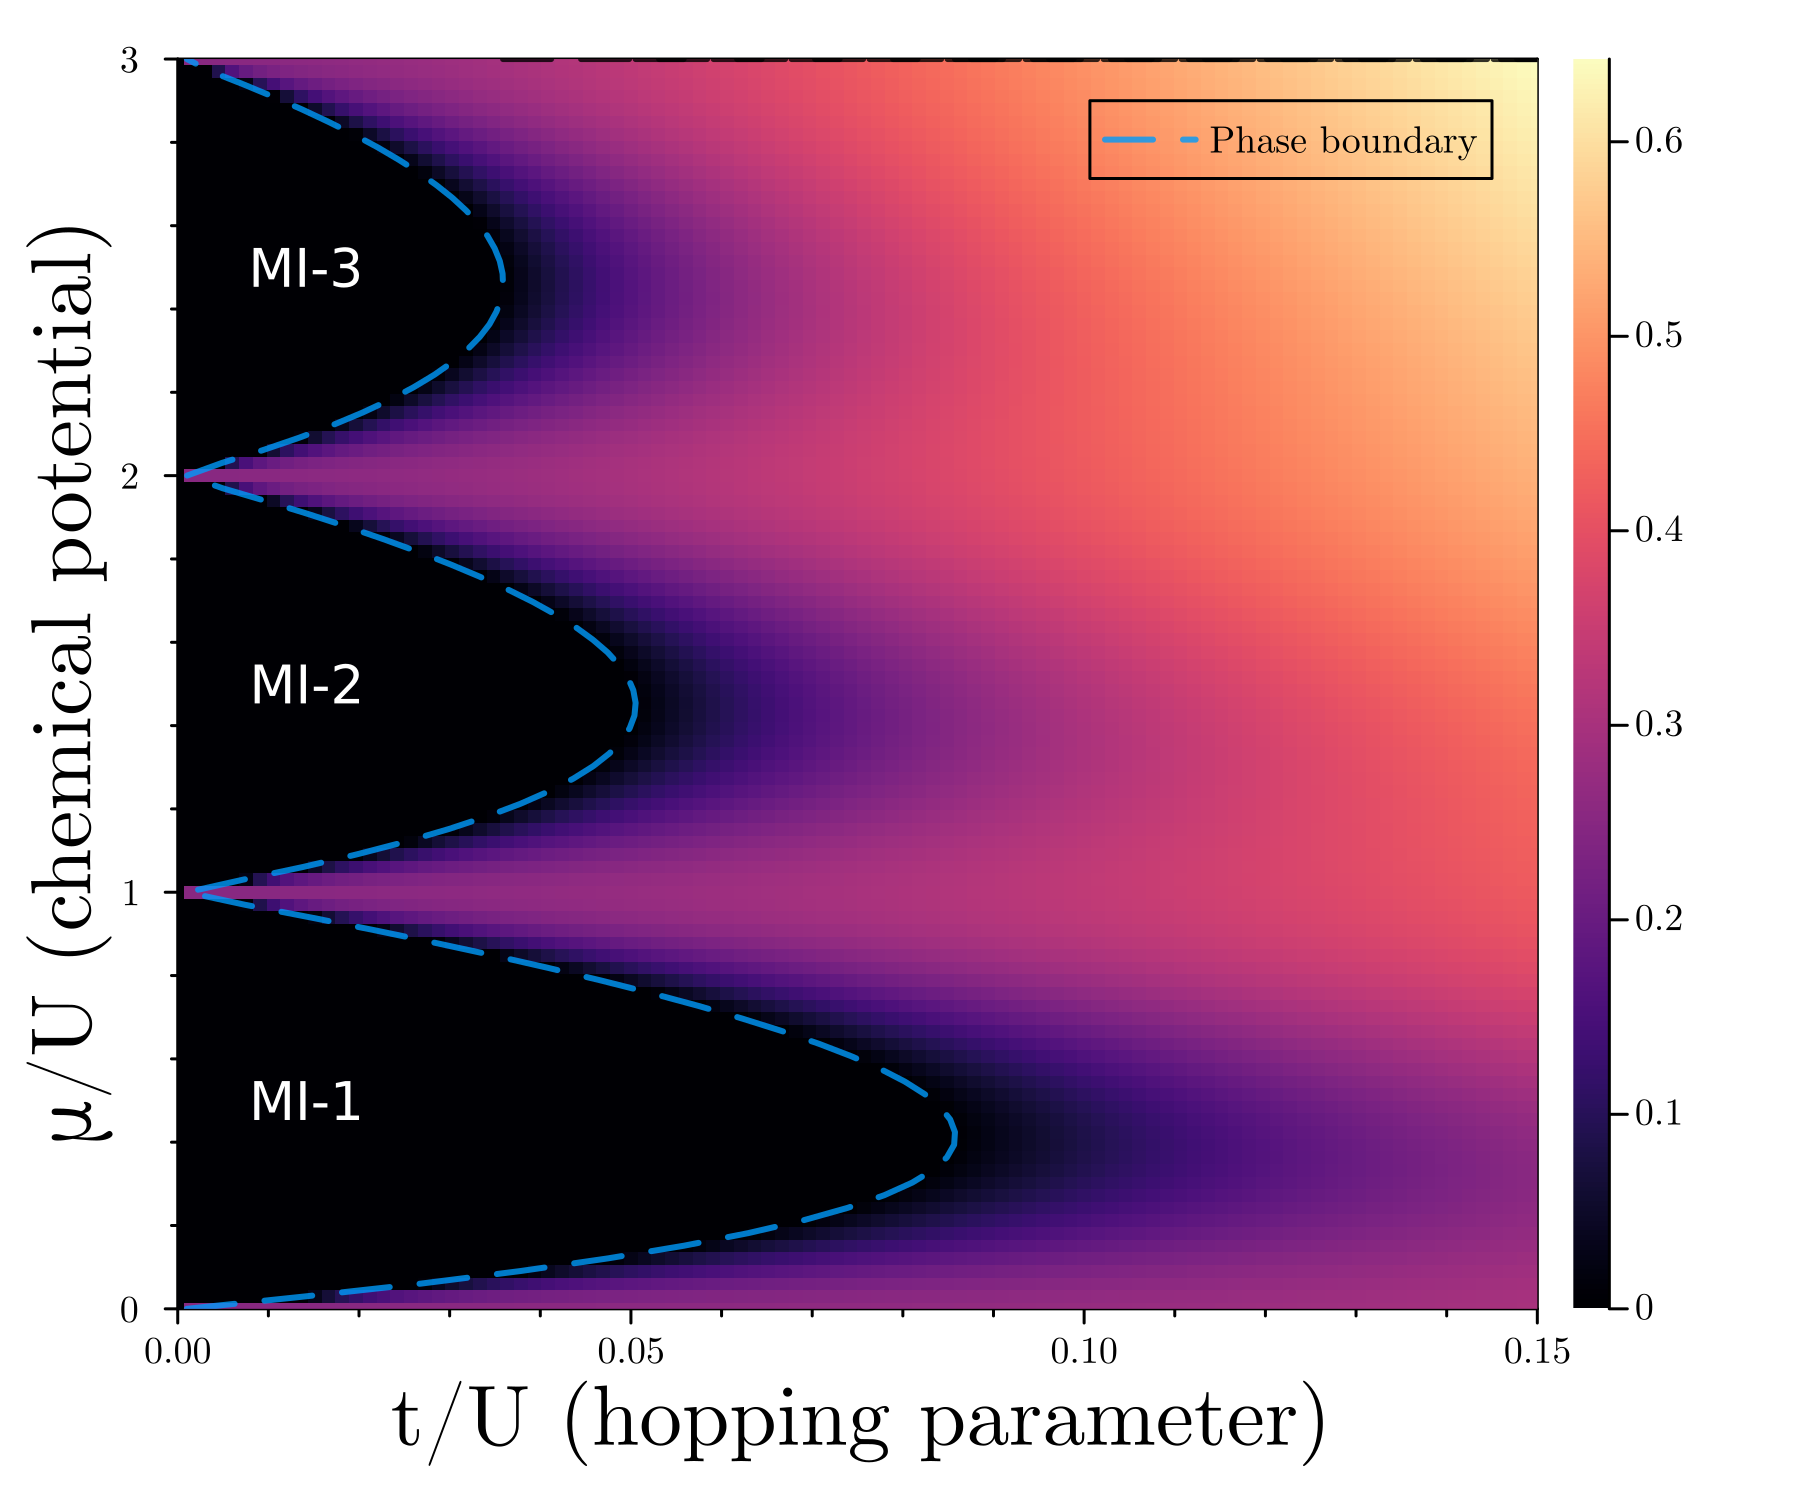
\includegraphics[width=\textwidth]{ch4/phase_diagram_nvar.png}
        \caption{Occupation number variance, $\langle \delta n^2 \rangle$}
        \label{fig:mft_occvar}
    \end{subfigure}
    \caption{1D Mean-field phase diagram}
    \label{}
\end{figure}
%%% FIG %%%
\FloatBarrier \!\!\!\!\!\!\!\!\!\!\!

A clean phase diagram is obtained in Fig \ref{fig:mft_pd}, where the Mott insulator phase manifests as lobes in the $t-\mu$ plane. We also note from Fig. \ref{fig:mft_occvar} that the occupation number variance serves as an equally valid order parameter, giving us the same phase boundary (although the heatmap is a bit misleading). We can now get further insight into the nature of the Mott lobes by plotting the average occupation number.
%%% FIG %%%
\begin{figure}[!htb]
    \centering
    \begin{subfigure}[b]{0.43\textwidth}  %keep total sum <1 to show in same line
        \centering
        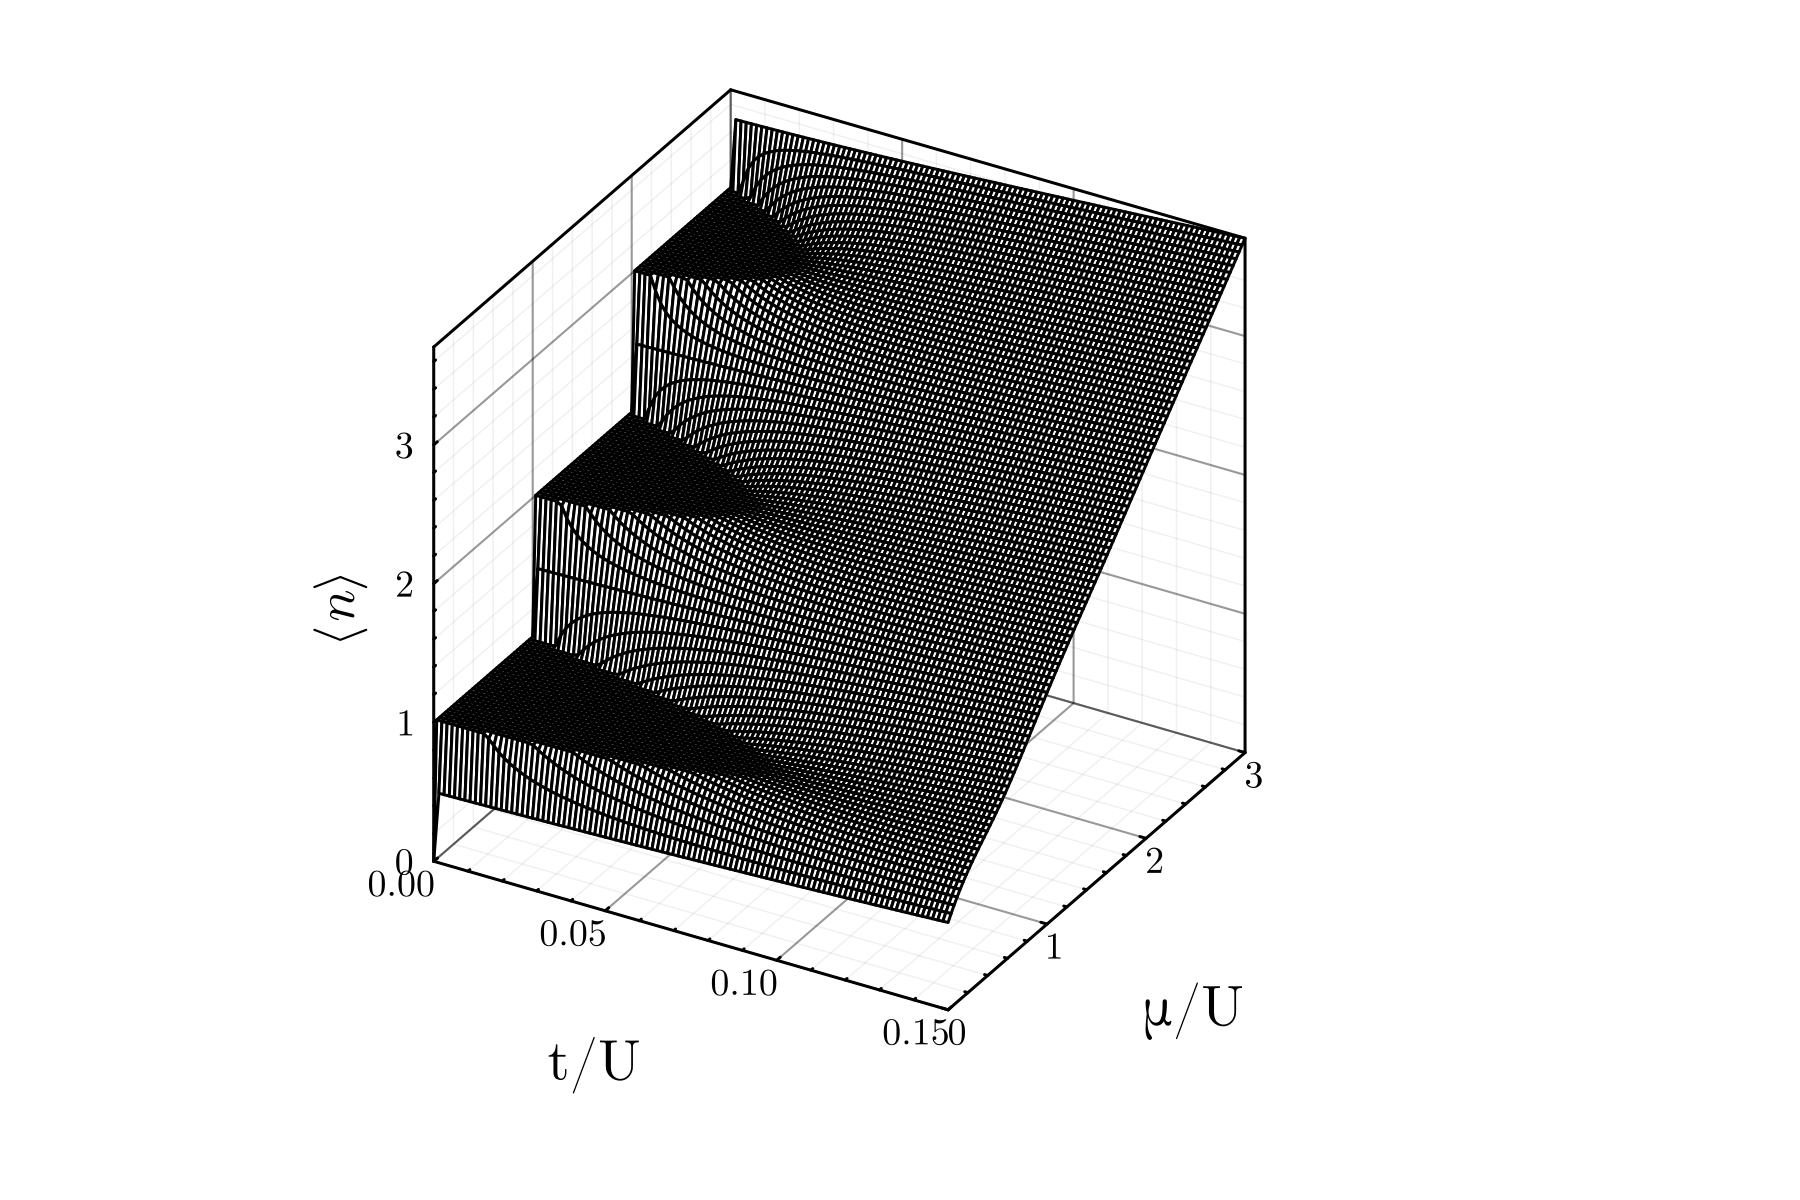
\includegraphics[width=\textwidth]{ch4/num_particles.png}
        \caption{Average occupation number}
    \end{subfigure}
    \hspace{1em}  %\hfill
    \begin{subfigure}[b]{0.4\textwidth}
        \centering
        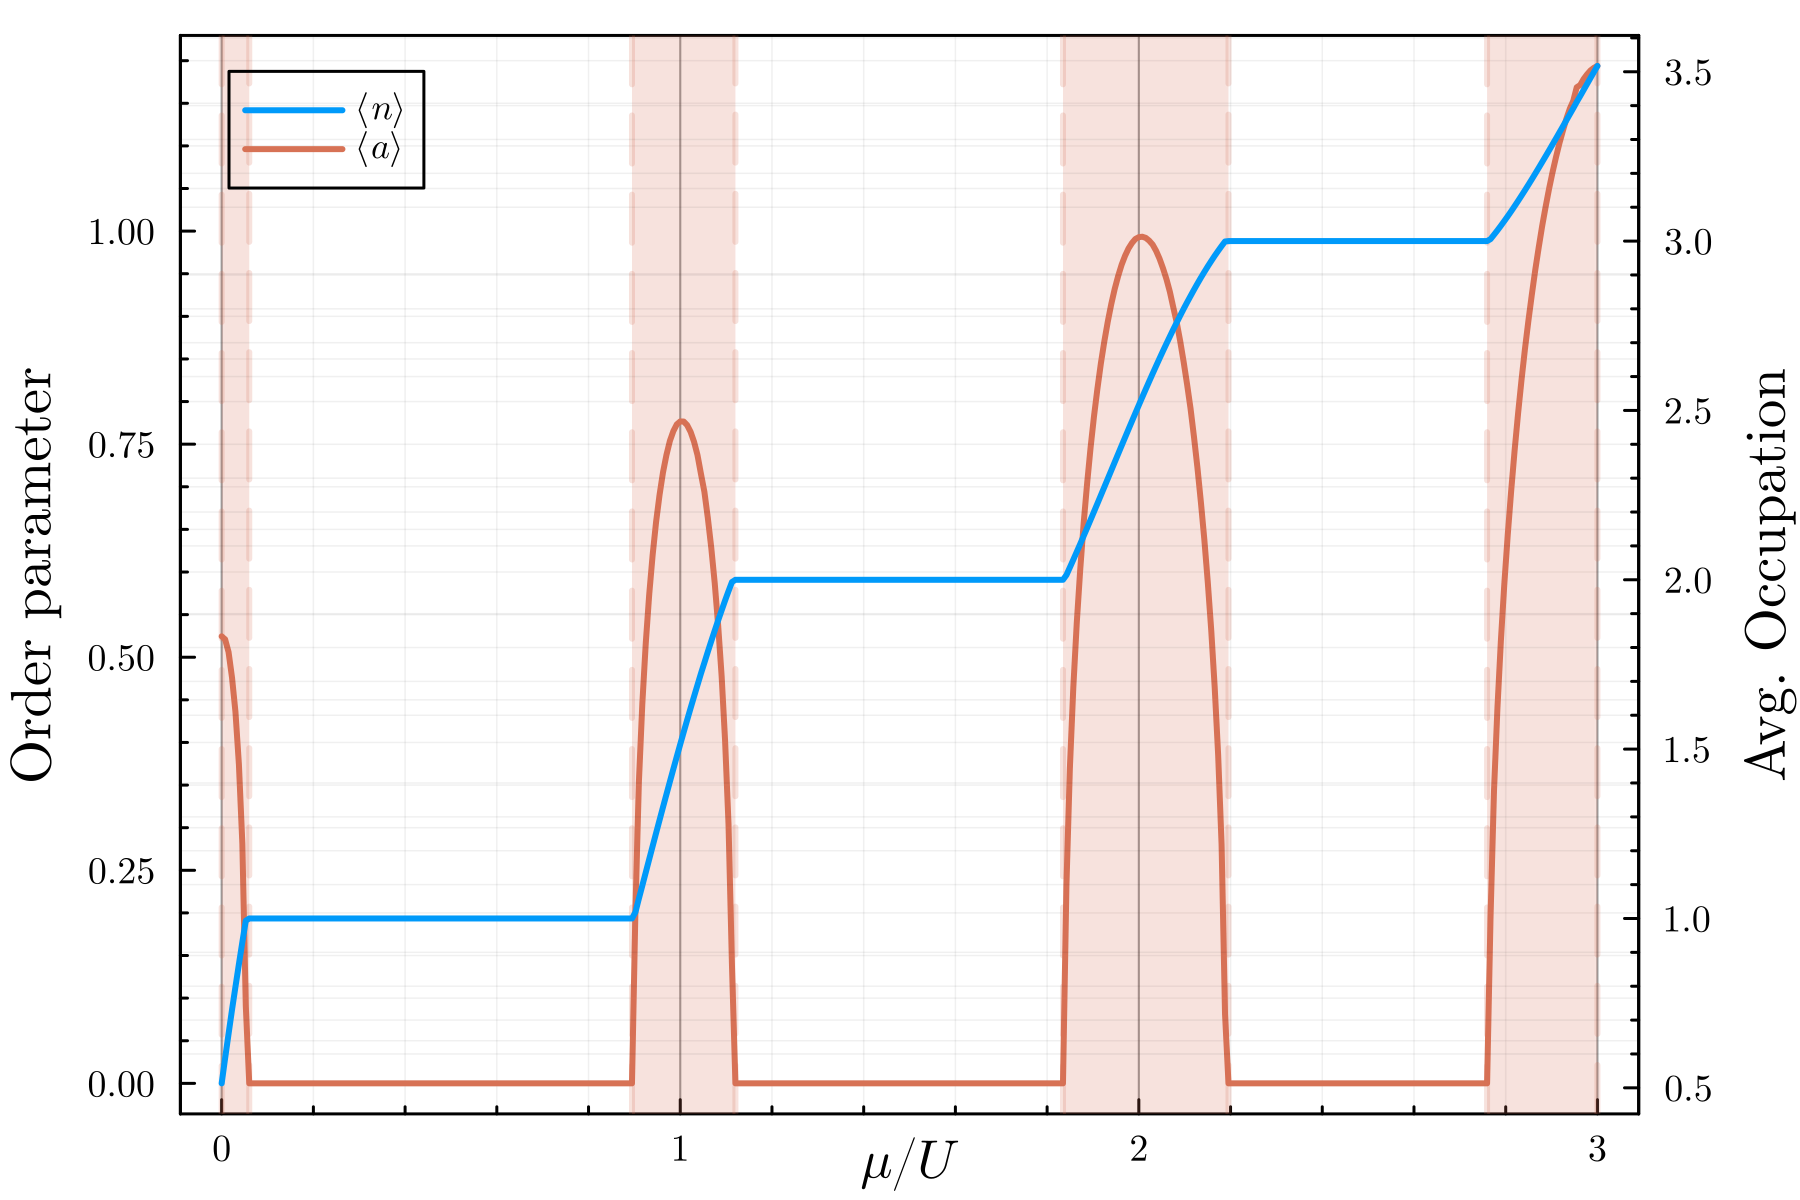
\includegraphics[width=\textwidth]{ch4/MFT_section.png}
        \caption{Cross-section at $t = 0.024$}
    \end{subfigure}
    \caption{Distinguishing phases using the average occupation}
    \label{fig:mft_avg_occ}
\end{figure}
%%% FIG %%%
\FloatBarrier \!\!\!\!\!\!\!\!\!\!\!

As expected, Fig. \ref{fig:mft_avg_occ} shows the existence of integer occupation plateaus corresponding to the points where the order parameter vanishes in the phase diagram. As the chemical potential is increased, there is a sudden jump to the next Mott lobe admitting one more boson per lattice site. Further, for a given point inside a Mott lobe, the vertical distance to the lower (upper) arm denotes the energy required to excite a hole (particle), thus supporting the fact that the Mott insulator is indeed a gapped phase. 
\vspace{0.5cm}\\
We also note that the MI-SF transition is second order since the order parameter changes continuously across the boundary. As a result, one can also perturbatively treat the hopping term in Eq. \ref{eq:mft} to directly obtain an analytic expression for the phase boundary\cite{Cubela19}. This matches exactly with our numerical results since the perturbative term is proportional to $\Psi$, which can be chosen to be arbitrarily small near the phase boundary. 

\subsection{A better technique}
Although the grid-based approach gives us a qualitative idea of the phase diagram, the accuracy of the phase boundary is limited by the discretization of the grid. However, the fact that there is only a single transition along $t$ for a fixed value of $\mu$ lets us utilize a bisection method to determine the transition point, $t_c$. Performing this for a grid of values of $\mu$ gives us the phase boundary such that the error falls as $1/2^n$ for $n$ bisections.
\vspace{0.5cm}\\
But we can do even better! To utilize the bisection method, at any given point we only require the information of the ground state phase, i.e, the rest of the information contained in the ground-state is unnecessary. One approach could be to directly check if $\Psi = 0$ is a fixed point of the self-consistency function in Eq. \ref{eq:self_fn}. However, it turns out that $\Psi=0$ is \textit{always} a fixed point, but is unstable for the superfluid phase. In order to find another approach, let us analyze the nature of convergence of the self-consistent procedure.
%%% FIG %%%
\begin{figure}[!htb]
    \centering
    \begin{subfigure}[b]{0.45\textwidth}  %keep total sum <1 to show in same line
        \centering
        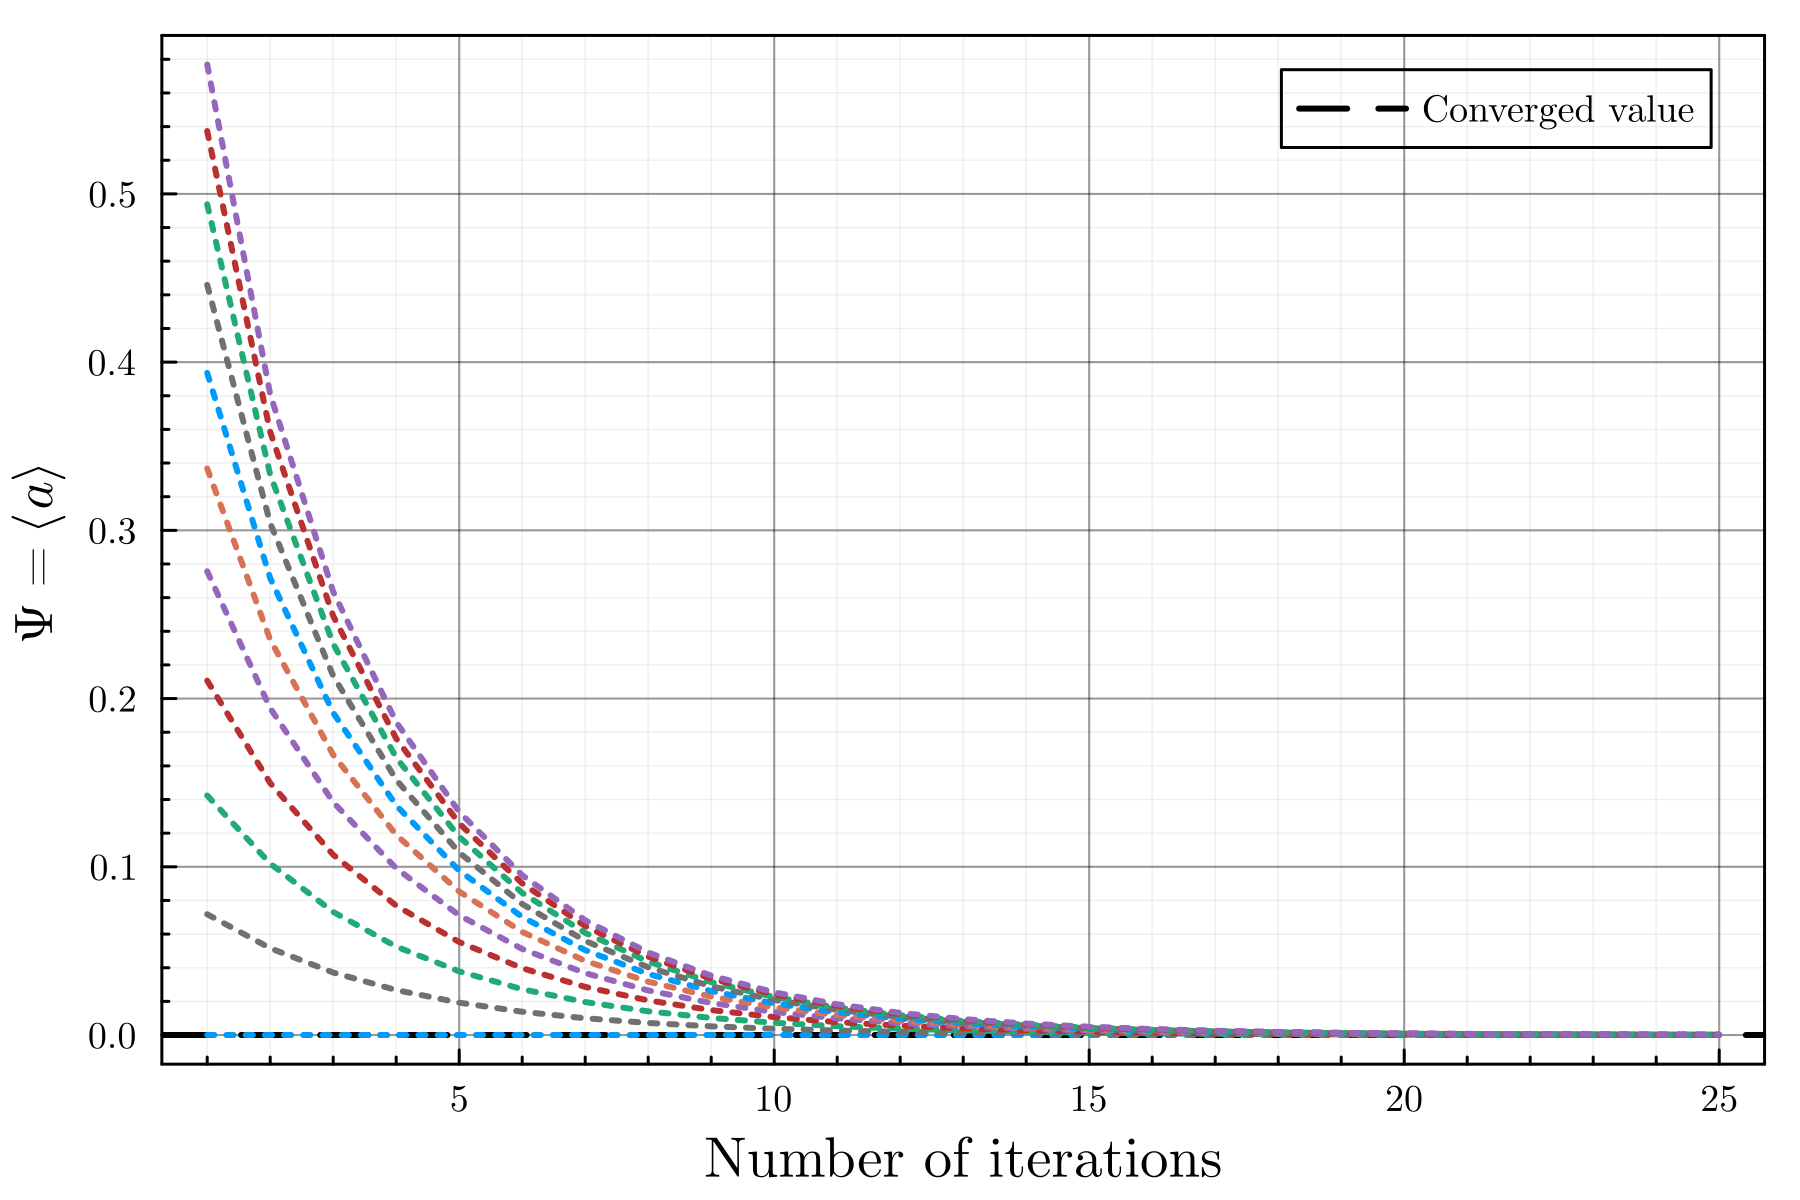
\includegraphics[width=\textwidth]{ch4/MI_converge.png}
        \caption{$t = 0.06, \mu = 0.5$}
    \end{subfigure}
    \hspace{1em}  %\hfill
    \begin{subfigure}[b]{0.45\textwidth}
        \centering
        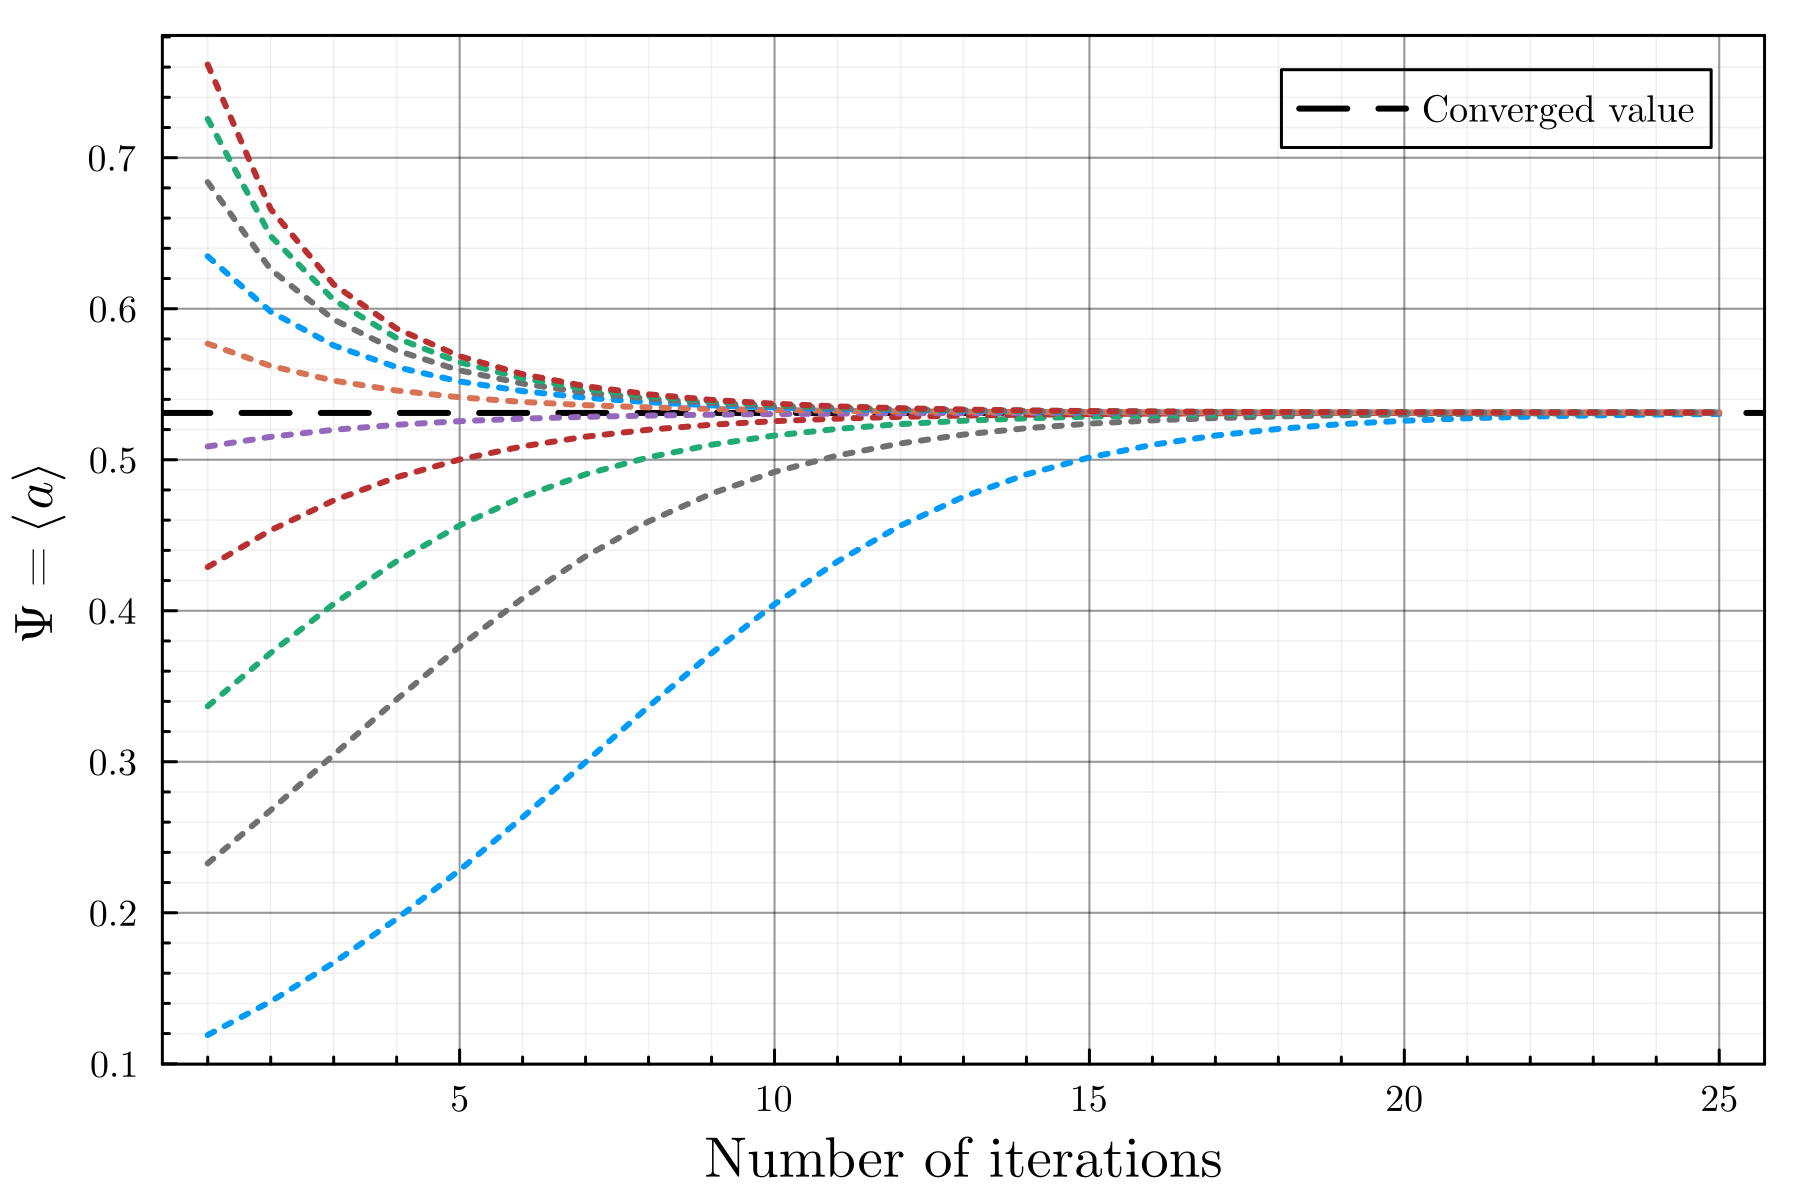
\includegraphics[width=\textwidth]{ch4/SF_converge.png}
        \caption{$t = 0.1, \mu = 0.5$}
    \end{subfigure}
    \caption{Monotonic convergence of self-consistency loop}
    \label{fig:self_consistent_converge}
\end{figure}
%%% FIG %%%
\FloatBarrier \!\!\!\!\!\!\!\!\!\!\!

It is apparent from Fig. \ref{fig:self_consistent_converge} that fixed-point iteration always monotonically converges to the stable fixed point for this system. This means that using a small initial guess such as $\Psi^{(0)} = 1\mathrm{e}{-9}$, we can determine whether $\Psi=0$ is a stable fixed point with a single iteration of the self-consistency loop\cite{Luhmann2013, Kho16}! 

%%% FIG %%%
\begin{figure}[!htb]
    \centering
    \begin{subfigure}[b]{0.75\textwidth}  %keep total sum <1 to show in same line
        \centering
        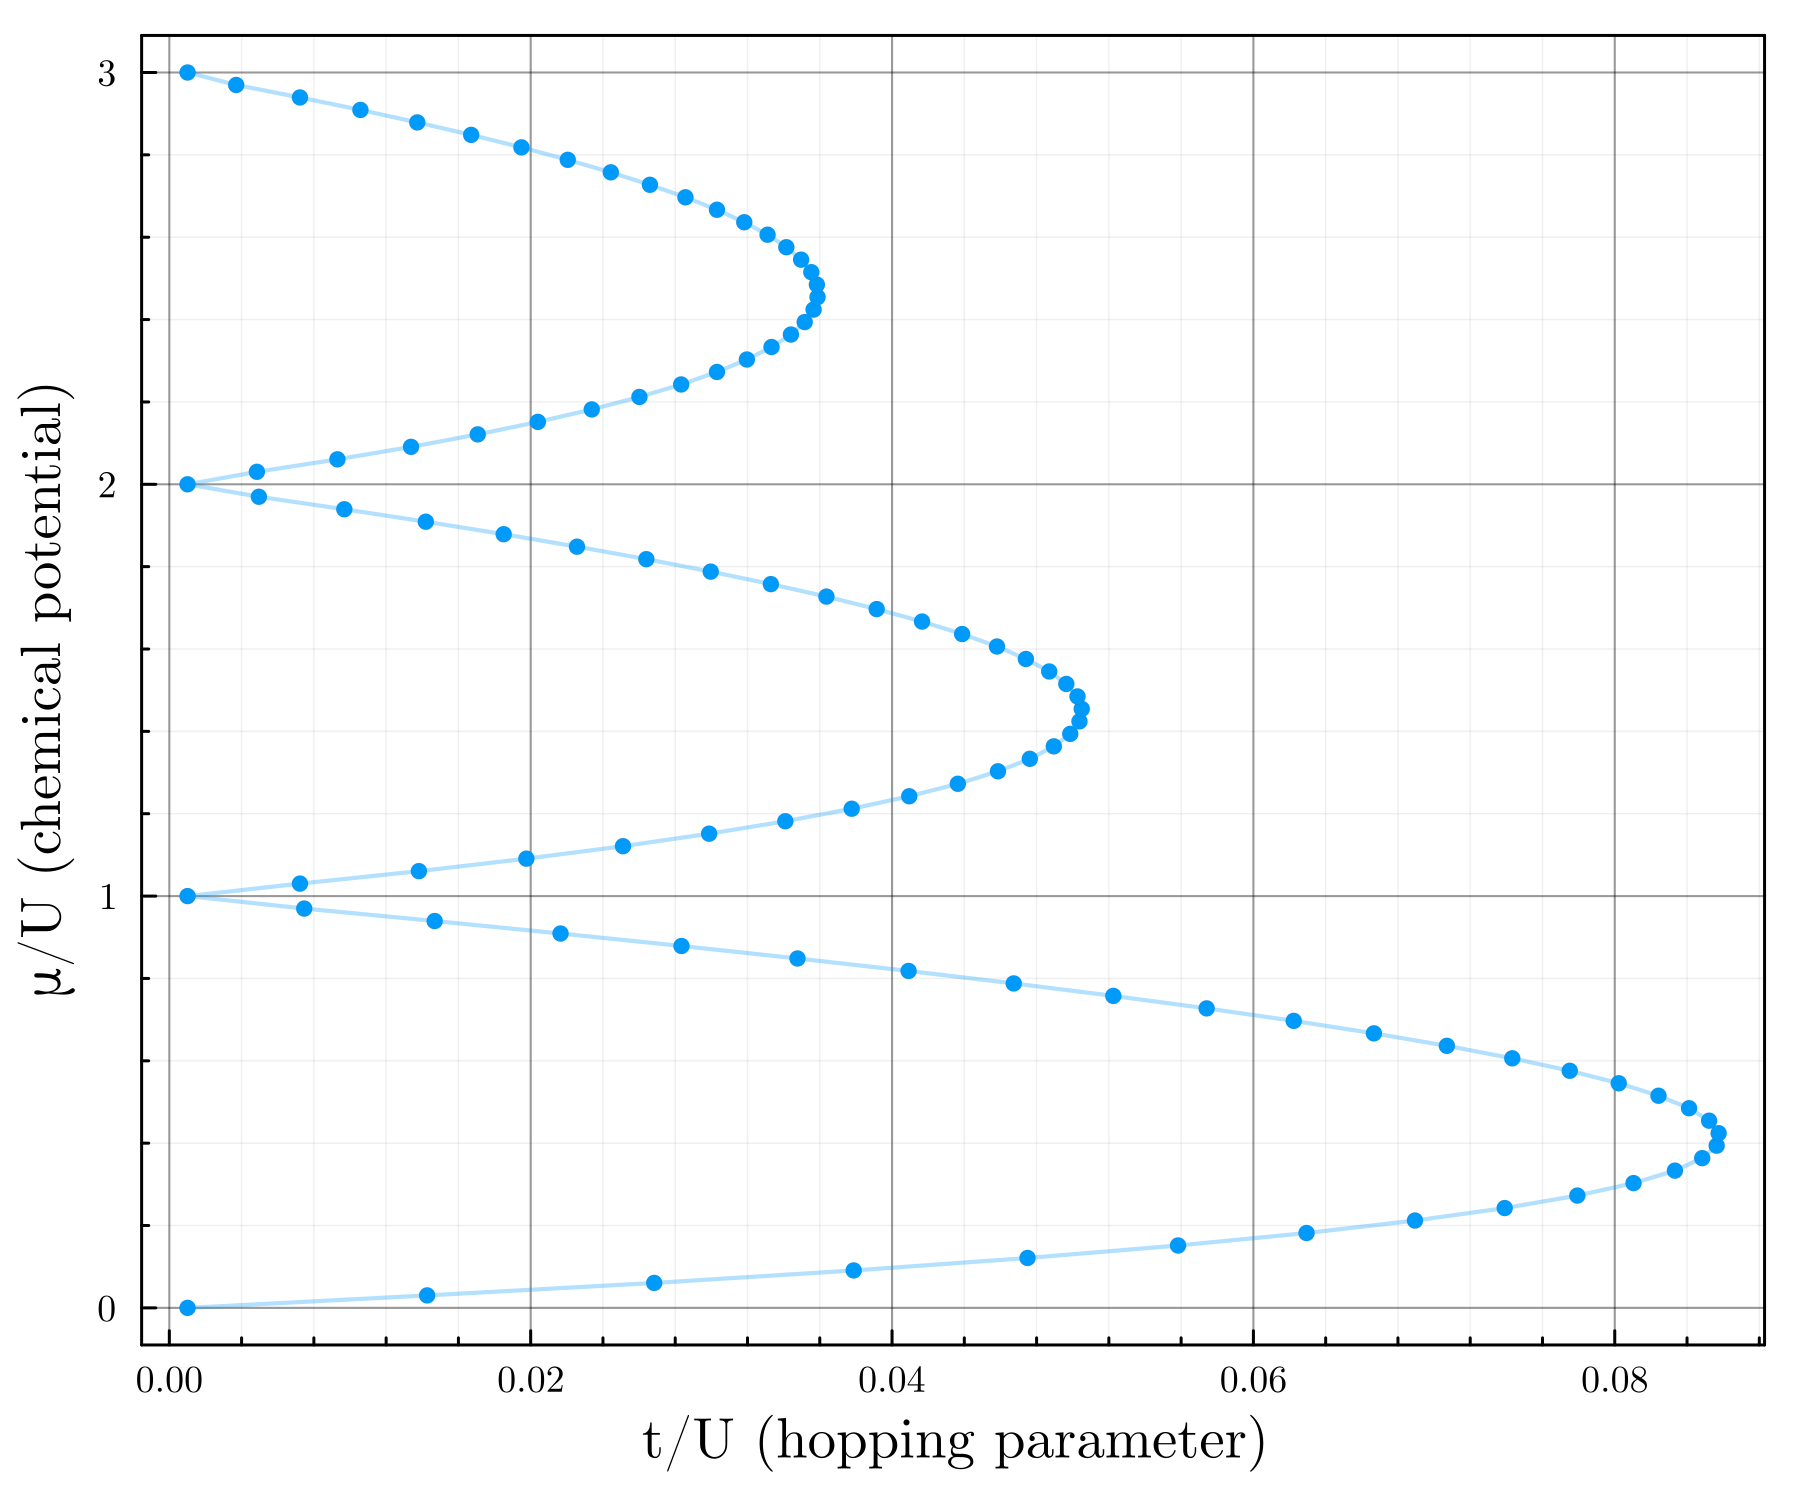
\includegraphics[width=\textwidth]{ch4/phase_diagram_bisection.png}
    \end{subfigure}
    \caption{1D Mean-field phase boundary determined by the bisection technique}
    \label{}
\end{figure}
%%% FIG %%%
\FloatBarrier \!\!\!\!\!\!\!\!\!\!\!

\subsection{Determining $n_{max}$}\label{sec:nmax}
Before wrapping up, we must tackle the issue of dealing with an infinite dimensional Hamiltonian. Truncating the Fock space at an arbitrary occupation number might seem like it fundamentally changes the model under consideration. The extreme limit of this is setting $n_{max} = 1$ corresponding to a system of hard-core bosons, and any higher truncation amounts to considering semi-hardcore bosons of sorts.
%%% FIG %%%
\begin{figure}[!htb]
    \centering
    \begin{subfigure}[b]{0.75\textwidth}  %keep total sum <1 to show in same line
        \centering
        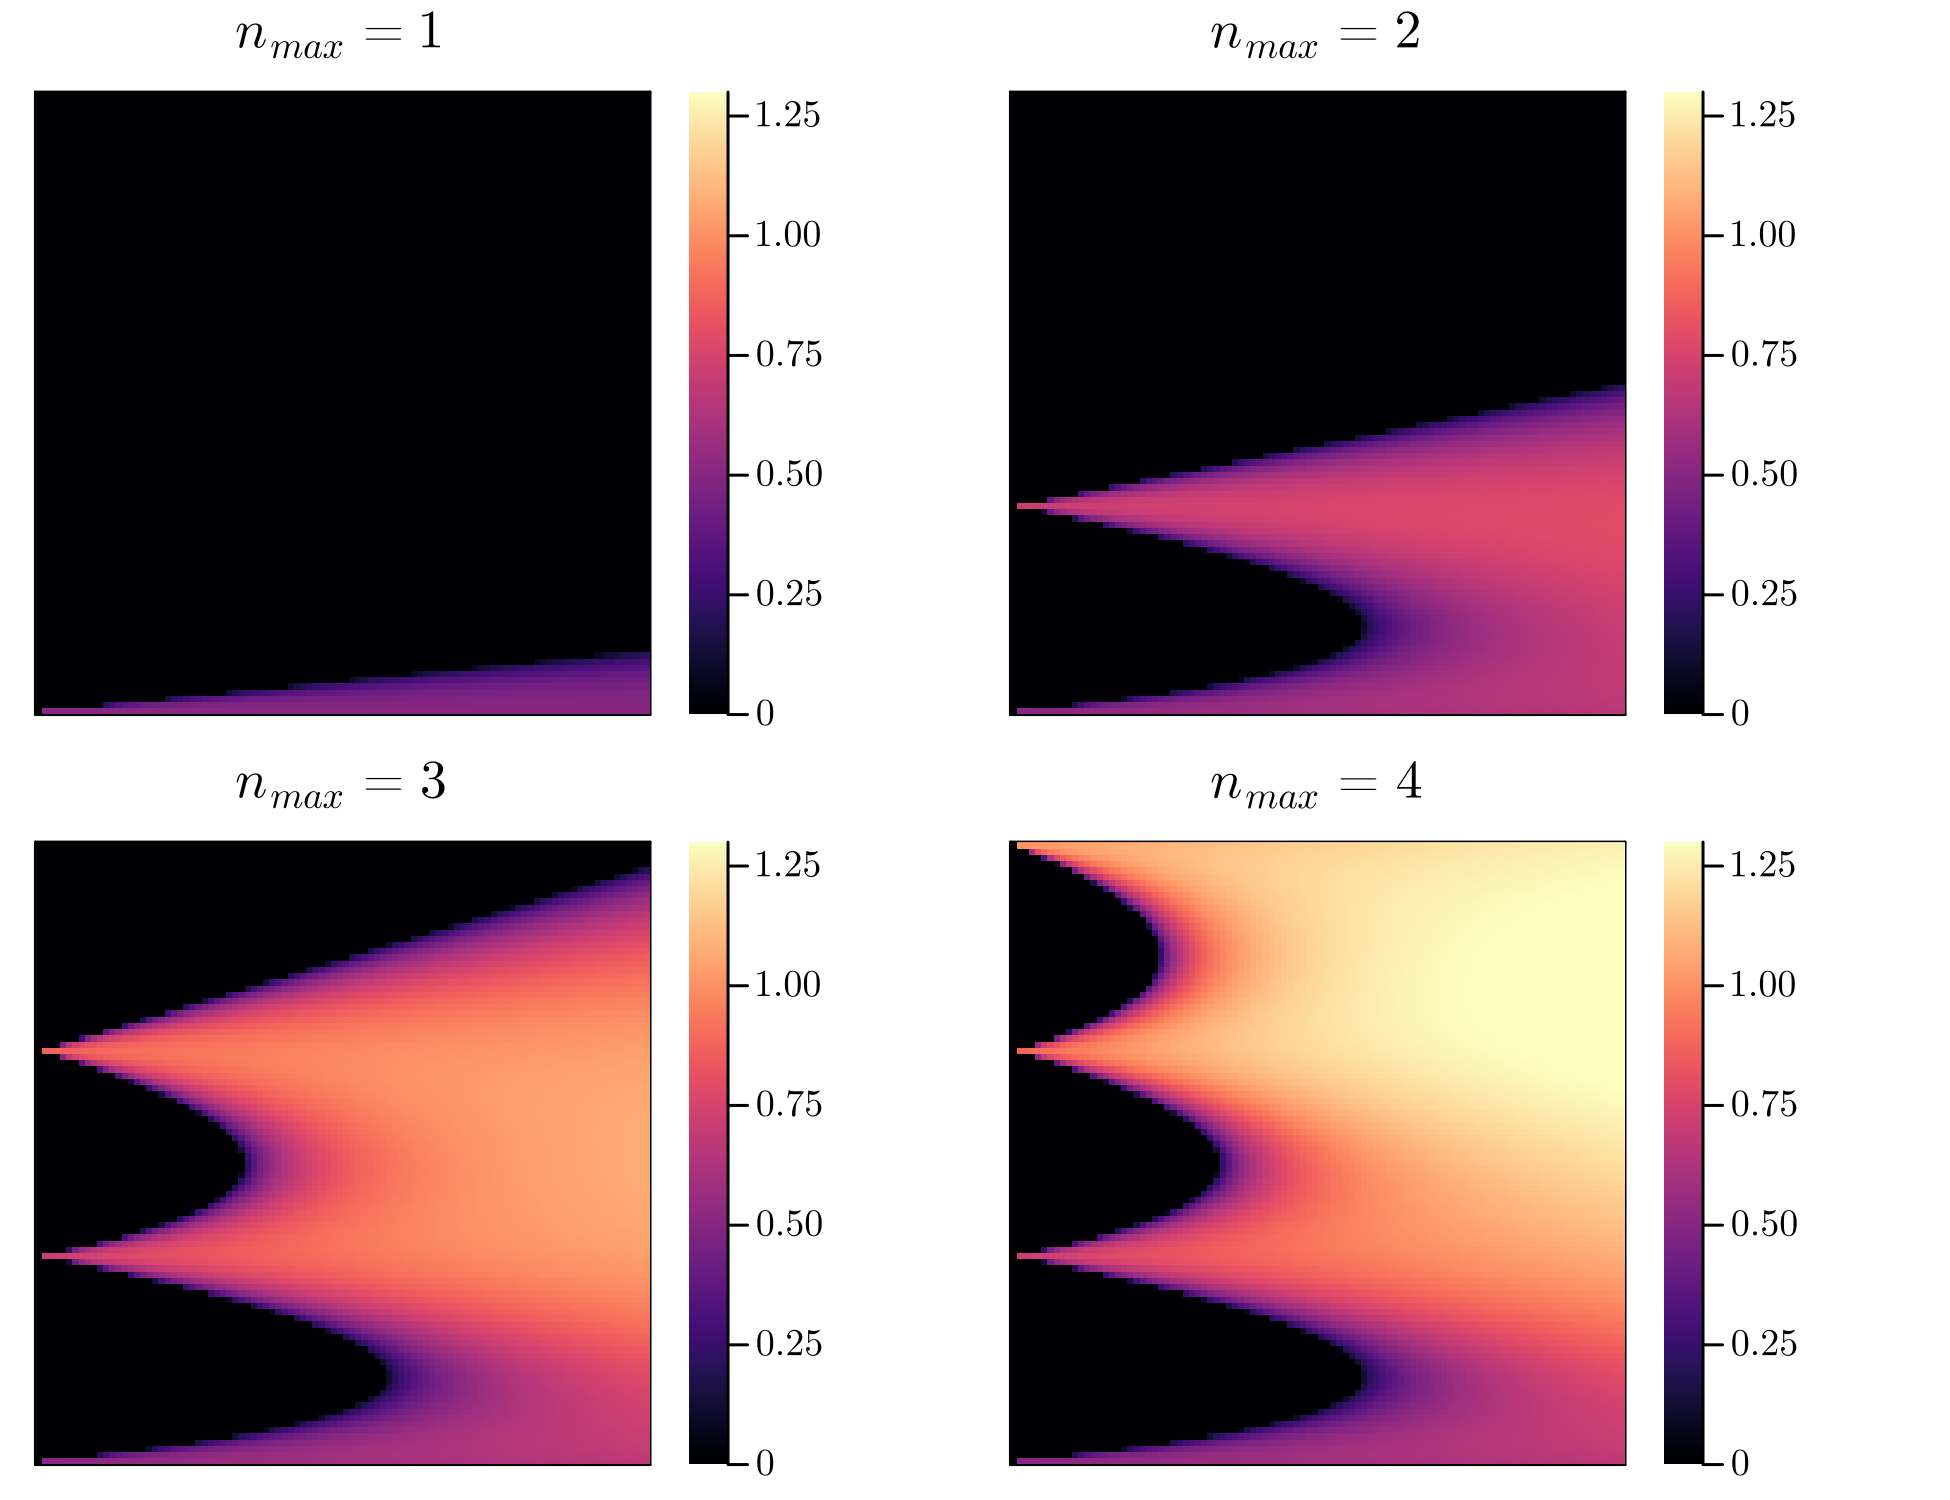
\includegraphics[width=\textwidth]{ch4/cutoff.png}
    \end{subfigure}
    \caption{Qualitative variation of phase diagram as the occupation cutoff is increased.}
    \label{fig:nmax}
\end{figure}
%%% FIG %%%
\FloatBarrier \!\!\!\!\!\!\!\!\!\!\!

Most notably, there will only be $n_{max}$ Mott lobes and for larger chemical potential, the entire parameter space will remain a Mott insulator since the maximum number of bosons is capped. However, we can see that this is a minor issue upon realizing that the physics of the low-energy lobes remain largely unaffected by the truncation and discrepancies only arise closer to the high-energy lobes. This is demonstrated in Fig. \ref{fig:nmax} and can be checked rigorously by quantifying the convergence of the phase boundaries as $n_{max}$ is increased.
\vspace{0.5cm}\\
In this thesis, we mostly focus on the first three Mott lobes, and the corresponding phase boundaries are found to converge quickly as $n_{max}$ is increased upto a value of 10.

\subsection{Extending to finite temperature}
In this section, we demonstrate that the mean-field approach is capable of handling finite temperature calculations as well. The only change required is to compute the expectation values as thermal expectations, by working with density matrices instead of the ground state. The self-consistency relation $\Psi = \langle \hat{a} \rangle_T = \Tr{\hat{a}\rho}/\Tr{\rho}$ can be recovered as well by imposing minimization of the free energy. 
%%% FIG %%%
\begin{figure}[!htb]
    \centering
    \begin{subfigure}[b]{\textwidth}  %keep total sum <1 to show in same line
        \centering
        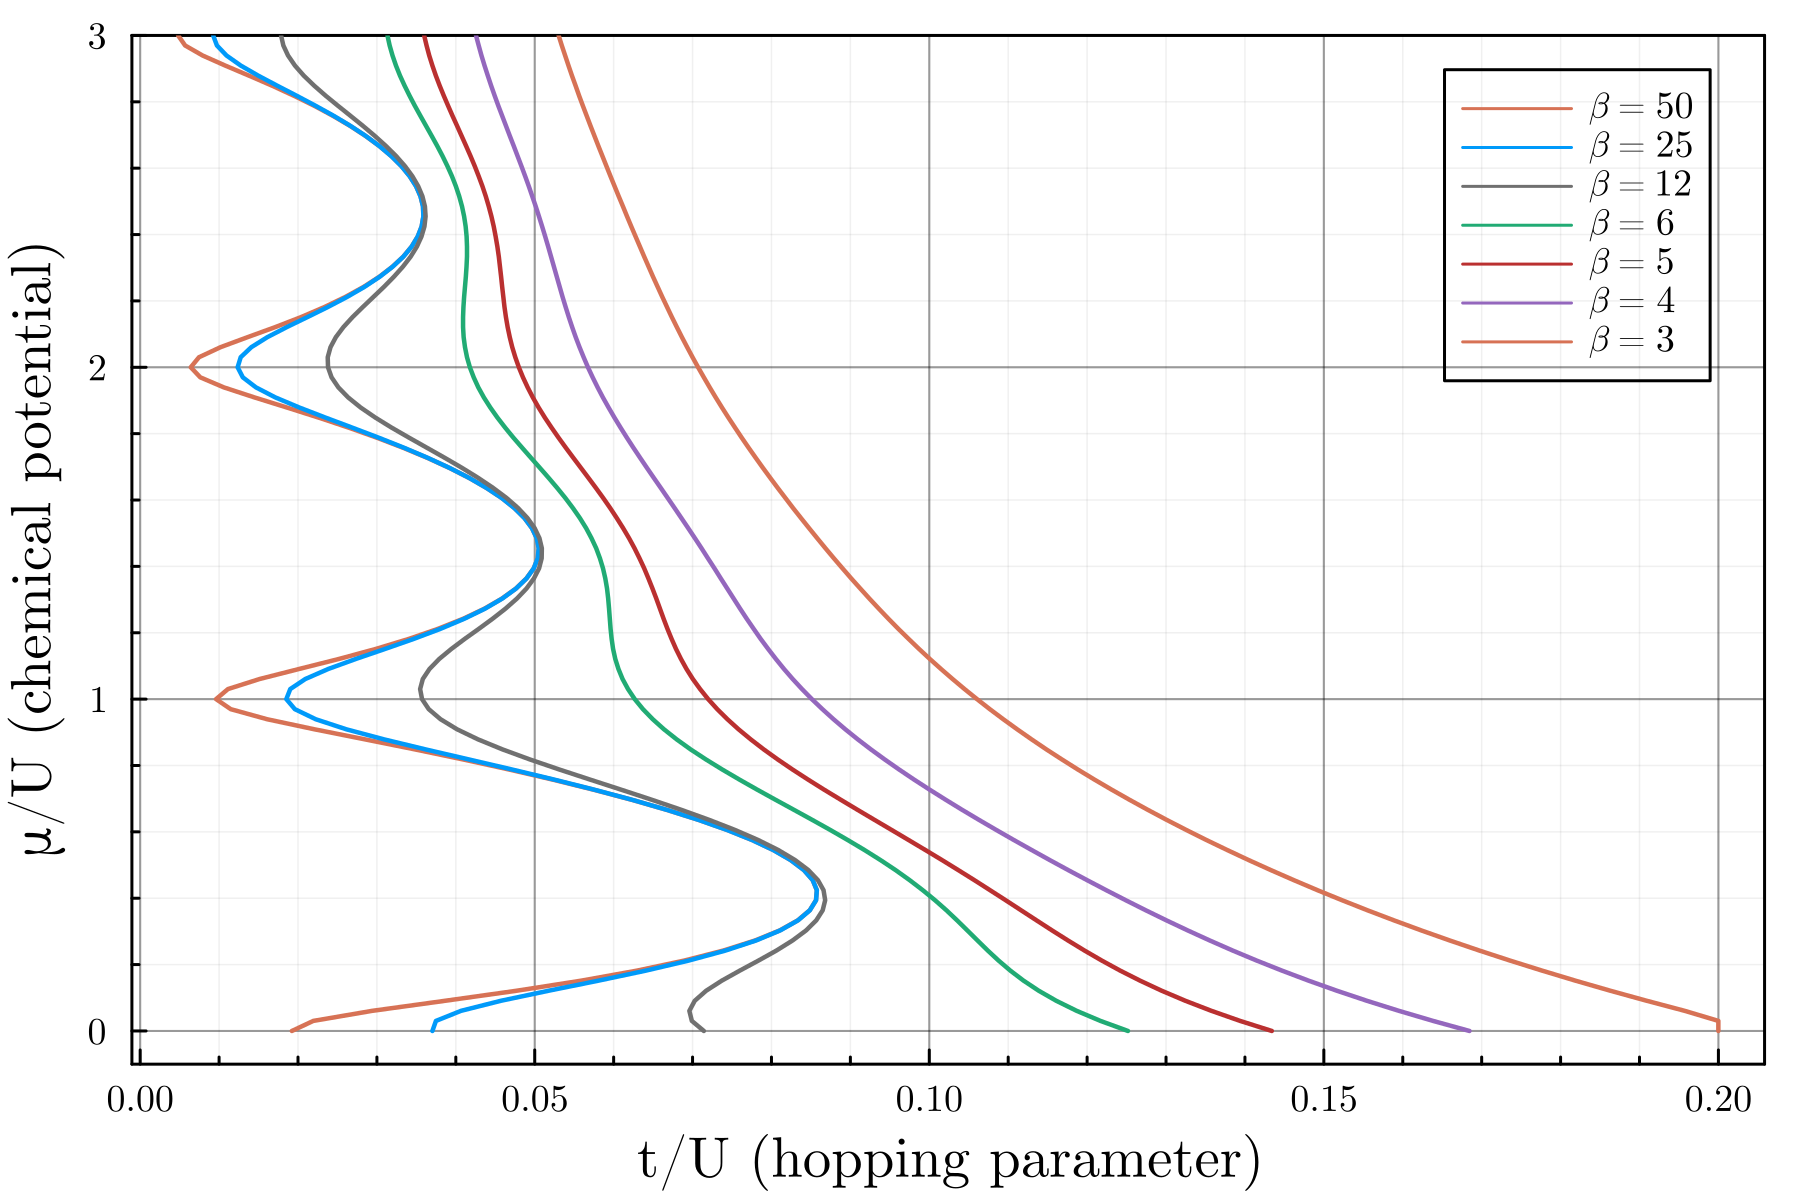
\includegraphics[width=\textwidth]{ch4/finite_temp.png}
    \end{subfigure}
    \caption{1D Mean-field phase boundaries at finite temperatures.}
    \label{fig:mft_temp}
\end{figure}
%%% FIG %%%
\FloatBarrier \!\!\!\!\!\!\!\!\!\!\!

At a finite temperature, Fig. \ref{fig:mft_temp} seemingly shows that the Mott insulator lobes coalesce into a single region as the temperature is increased. However, this is infact due to the formation of a thermally disordered phase, namely, the normal fluid. At the mean field level, it seems similar to the superfluid since it has finite compressibility and variance of occupation number. However, such a phase does not does not break the $U(1)$ symmetry and its formation is not driven by quantum fluctuations. 
\vspace{0.5cm}\\
As the temperature is increased, the Mott insulator lobes start vanishing and the extent of the superfluid region decreases as the normal fluid becomes the most stable phase throughout the parameter space. 

\subsection{An alternative de-coupling}
Decoupling the hopping term ($a_i^{\dagger}a_j$) seems ubiquitous in literature when trying to simplify the Bose-Hubbard model. Strangely, the standard scheme for the mean-field study of the (fermionic) Hubbard model involves decoupling the interaction term instead. Nothing stops us apriori from utilizing a similar scheme as well. 
\begin{align}
    &\hspace{1.2cm}\hat{n}_i = \rho_i + \delta \hat{n}_i \nonumber\\
    &\implies \delta n_i^2 = (n_i - \rho_i)(n_i - \rho_i) \approx 0 \nonumber\\
    &\implies n_i^2 \approx 2\rho_i n_i - \rho_i^2
\end{align}
The Hamiltonian can then be written as:
\begin{equation}
    H_{MF} = -t\sum_{\langle i, j \rangle} a_i^{\dagger} a_j + \sum_i \left( \mu - \frac{U}{2} + U\rho_i\right) n_i - \frac{U}{2}\sum_i \rho_i^2
\end{equation}
If we utilize translational symmetry to set $\rho_i = \rho$ and switch to the Bloch basis, we get:
\begin{equation}
    H_{MF} = -t\sum_{k} \left(\epsilon_k + \mu - \frac{U}{2} + U\rho\right) \tilde{a}_k^{\dagger} \tilde{a}_k - \frac{U}{2}M\rho^2
\end{equation}
Since this is already diagonal, the ground state would simply be a condensate in the $k$-mode with lowest energy. Note that such a decoupling still preserves the conservation of particle number and as a result, $\langle a \rangle$ can no longer serve as an order parameter for the superfluid phase. Regardless, we see that a Mott insulator can never be admitted as a ground state by such a Hamiltonian since it is always a condensate. This exercise brings to light an apparent subjectivity involved in choosing an appropriate decoupling. However, although the choice may be guided by considering the limiting behaviour of the system, the right choice is the one that generates the lowest ground state energy. Such a claim can be made rigorous if we view the mean field treatment as a variational method\cite{sachdev_2011}.

\subsection{Pitfalls}
Although the mean-field approach has allowed us to gain some insight on the BHM, it is only reliable for qualitative results. Particularly, since we have ignored higher order quantum fluctuations, we tend to over-estimate the extent of the ordered phase. Further, most of the information about the lattice geometry and dimensionality is lost as we only take into account the co-ordination number of each lattice site. Such a treatment only becomes exact in the limit of an infinite-dimensional lattice geometry. We will now proceed to formulate a numerical technique that tackles these issues.

\section{Cluster Mean Field Theory}
This technique can be seen a middle ground between exact diagonalization and single-site mean field theory as portrayed in Fig. \ref{fig:cmft_diagram}.
%%% FIG %%%
\begin{figure}[!htb]
    \centering
    \begin{subfigure}[b]{\textwidth}  %keep total sum <1 to show in same line
        \centering
        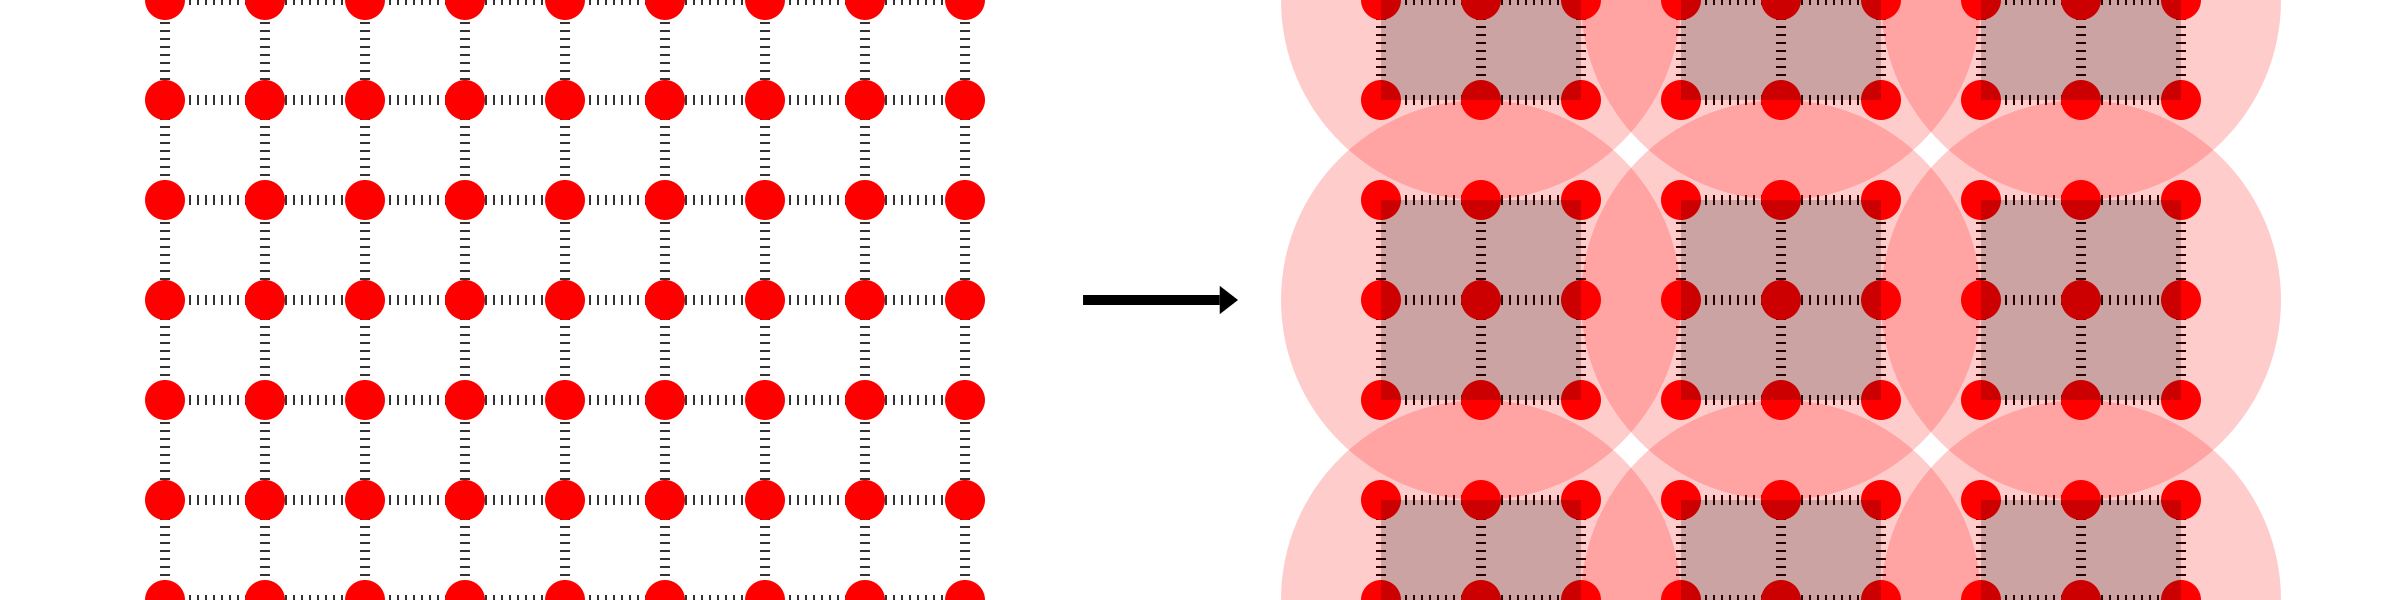
\includegraphics[width=\textwidth]{ch4/CMFTdiagram.png}
    \end{subfigure}
    \caption{Pictorial representation of CMFT in 2D}
    \label{fig:cmft_diagram}
\end{figure}
%%% FIG %%%
\FloatBarrier \!\!\!\!\!\!\!\!\!\!\!

 We demonstrate the idea by considering a 1D lattice with $M$ sites. The chain can then be divided into $N_c$ clusters, each of length $L$ such that $M = LN_c$. The hopping term of the BHM can now be written as follows.
 \begin{equation}
    H_{hop} = -t\sum_{j=0}^{N_c - 1}\sum_{l = 1}^{L-1} (a_{Lj+l}^{\dagger}a_{Lj+l+1} + a_{Lj+l + 1}^{\dagger}a_{Lj+l}) - t\sum_{j=0}^{N_c-1}(a_{Lj+L}^{\dagger}a_{Lj+L+1} + a_{Lj+L+1}^{\dagger}a_{Lj+L})
 \end{equation}
where the first term, $H_{\text{intra}}$ couples the sites within each cluster, and the second term, $H_{\text{inter}}$ couples the different clusters. The main idea of CMFT is to treat the intra-cluster coupling exactly and the inter-cluster coupling at a mean-field level. Following the same de-coupling we used in Eq. \eqref{eq:decoupling_scheme}, we obtain:
\begin{equation}
    H_{\text{intra}} = -t \sum_{j=0}^{N-1}[(a_{Lj+L}^{\dagger} + a_{Lj+L+1}^{\dagger})\Psi + (a_{Lj+L} + a_{Lj+L+1})\Psi^*] + 2tN_c|\Psi|^2
\end{equation}
where $\Psi = \langle a_i \rangle$ is the mean-field order parameter. Putting all this together, we arrive at the cluster-decoupled Hamiltonian.
\begin{equation}
    H_{MF}\{\Psi\} = \sum_{j=0}^{N_c-1} H_{MF}^L\{\Psi\} = \sum_{j=0}^{N_c-1} (H_j^L + V_j^L\{\Psi\})
\end{equation}
\begin{equation}
    H_j^L = -t\sum_{l=1}^{L-1}(a_{Lj + l}^{\dagger}a_{Lj + l+1} + a_{Lj + l+1}^{\dagger}a_{Lj + l}) + \frac{U}{2}\sum_{l=1}^L n_{Lj + l}(n_{Lj + l} - 1) - \mu \sum_{l=1}^L n_{Lj + l}
\end{equation}
\begin{equation}
    V^L_j\{\Psi\} = -t(\Psi(a_{Lj + 1}^{\dagger} + a_{Lj + L}^{\dagger}) + \Psi^*(a_{Lj + 1} + a_{Lj + L})) + 2t|\Psi|^2    
\end{equation}
Again, without loss of generality one can assume $\Psi \in \mathbb{R}$ and solve the system in a self-consistent manner. This procedure mostly remains the same for higher dimensions\cite{McIntosh_2012} and other lattice geometries\cite{Malakar_2020, Malakar_2023} but requires more book-keeping as we are forced to include more mean-field parameters (one for each distinct kind of boundary site in the cluster). 
\newpage
\subsection{Results}

%%% FIG %%%
\begin{figure}[!htb]
    \centering
    \begin{subfigure}[b]{0.6\textwidth}  %keep total sum <1 to show in same line
        \centering
        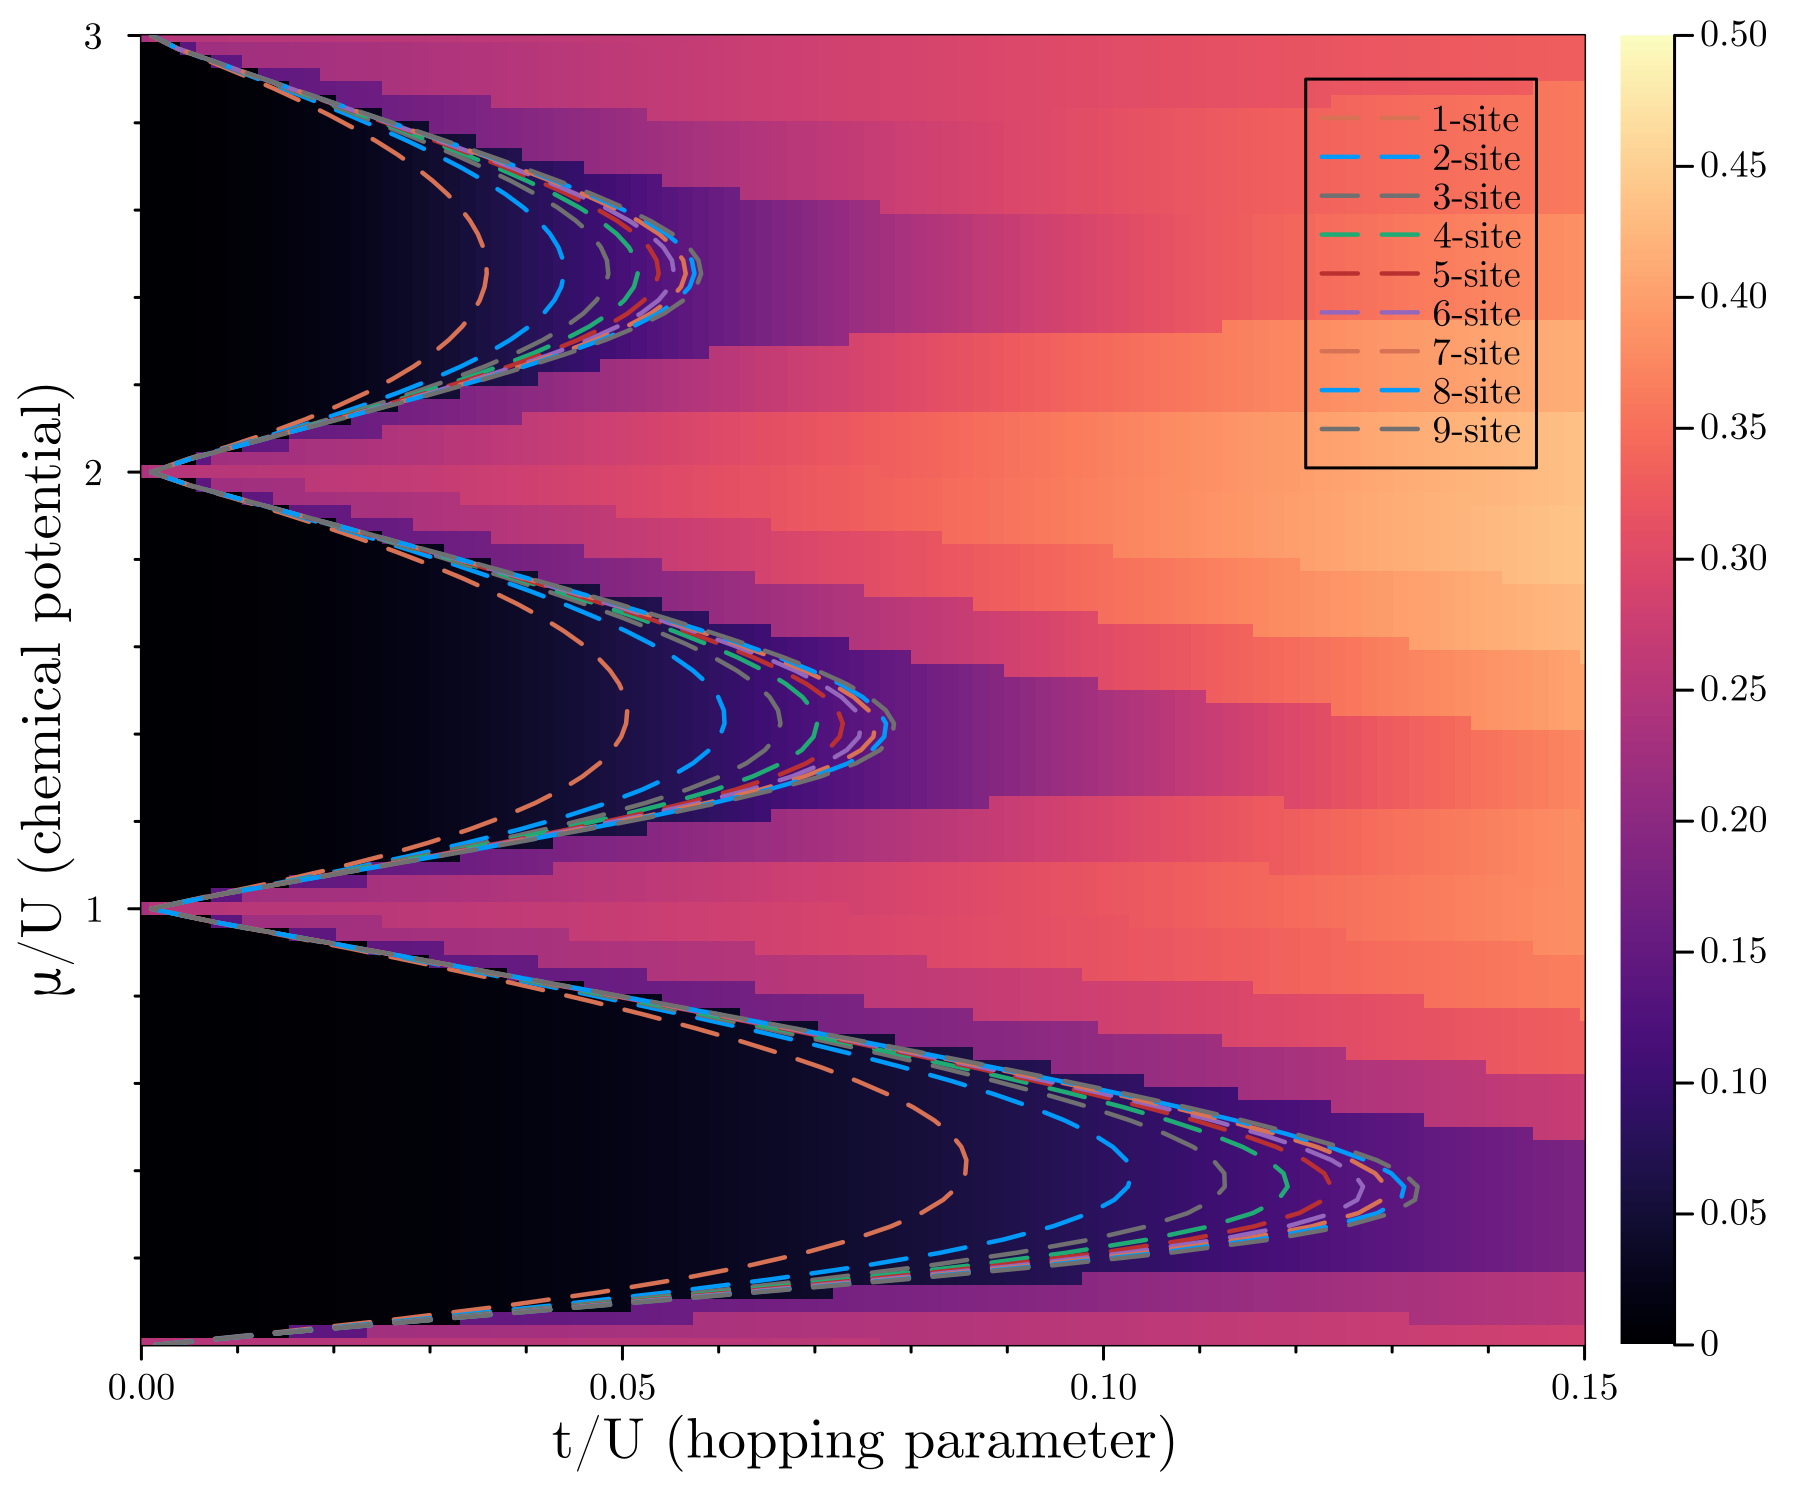
\includegraphics[width=\textwidth]{ch4/phase_diagram_cmft.png}
        \caption{Phase boundary}
    \end{subfigure}
    \hspace{1em}  %\hfill
    \begin{subfigure}[b]{0.3\textwidth}
        \centering
        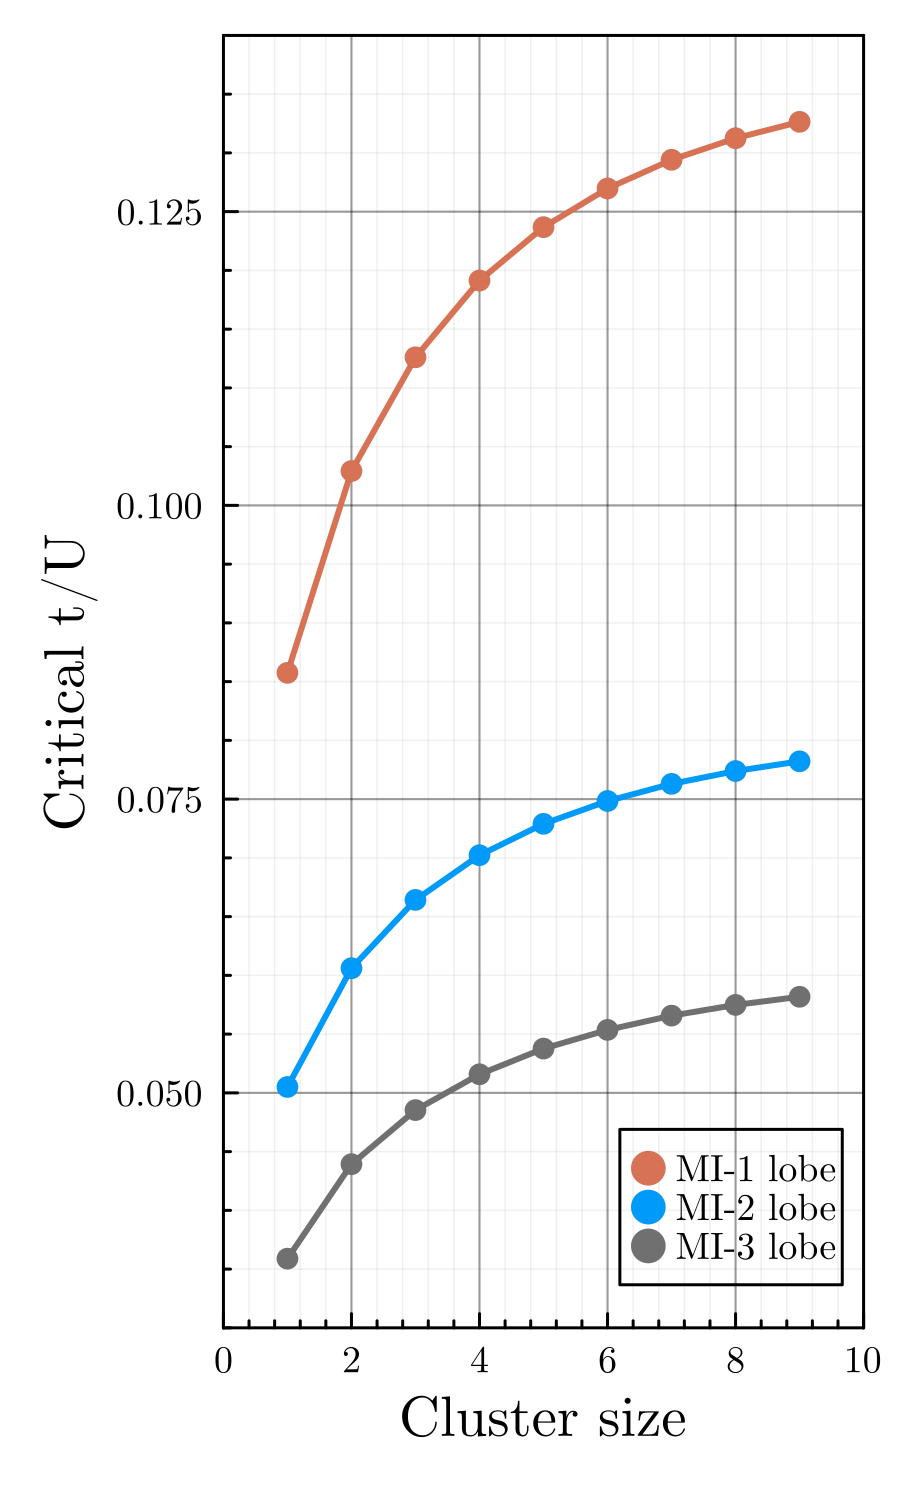
\includegraphics[width=\textwidth]{ch4/cmft_crit.png}
        \caption{Critical point of Mott lobes}
    \end{subfigure}
    \caption{Comparison of 1D CMFT results for various cluster sizes. The heatmap indicates the variance of occupation number obtained through exact diagonalization of the system with $M=6$ and $N_{max}=4$.}
    \label{}
\end{figure}
%%% FIG %%%
\FloatBarrier \!\!\!\!\!\!\!\!\!\!\!

We see that the estimation of the phase boundaries improves as we increase the size of the cluster. However, while the computational cost still grows exponentially, the marginal improvement of the boundary estimate diminishes for larger cluster sizes. Although this might only be the case for 1D systems, we decide not to employ this technique for further analysis due to the complexity involved in an implementation for arbitrary lattice geometries. 